\documentclass{foi}
\usepackage{lipsum}
\usepackage[utf8]{inputenc}
\usepackage{float}

\lstset{basicstyle=\ttfamily,
  showstringspaces=false,
  commentstyle=\color{red},
  keywordstyle=\color{blue},
}

\vrstaRada{\zavrsni}
\title{Izrada aplikacije za pronalazak termina sastanaka}

\author{Leo Ćavar}
\spolStudenta{\musko}
\mentor{Marko Mijač}
\spolMentora{\musko}
\godina{2024}
\mjesec{Rujan}
\date{2024}
\status{redoviti}
\indeks{0016153823}
\smjer{Informacijski i poslovni sustavi}
\titulaProfesora{Doc. Dr. sc.}

\sazetak{U ovom završnom radu se obrađuje korištenje .NET tehnologija za izradu programa za dogovaranje sastanka. Kroz rad se obrađuje kratko o ASP. NET Core i ASP. NET Web API tehnologijama, kao i koncepte API-ja i HTTP metoda, Google API-ja, uključujući Google Calendar API, autentifikaciju i autorizaciju korisnika pomoću OAuth 2.0 protokola, te primjere zahtjeva za dohvaćanje i upravljanje kalendarskim događajima kroz implementaciju .NET web aplikacije 
}

\kljucneRijeci{API; ASP. NET Core; .NET; C\#; ASP. NET; ; OAuth 2.0; Google Calendar; Google API;}

\begin{document}

\maketitle

\tableofcontents

\pagestyle{plain}
\chapter{Uvod}
U ovom radu ćemo se usredotočiti na izradu programa za dogovaranje sastanaka kroz upotrebu Google API-ja, koji nam omogućava interakciju s iznimno popularnim Google kalendarom. Realizirat ćemo program koristeći ASP.NET Core i Razor stranice za izradu front-end sučelja te upravljanje podacima, dok će ASP.NET Web API služiti za primanje HTTP zahtjeva i komuniciranje s Google servisima za manipuliranje događajima.

\chapter{Metode i tehnike rada}
Za pisanje teksta i formatiranje ovog rada koristio se LaTeX unutar programa Visual Studio Code. Za izradu praktičnog dijela korišten je Visual Studio 2022.

\chapter{GNU/Linux}
Linux je naziv jezgre (engl. \textit{kernel}) koju je razvio Linus Torvalds te čiji je izvorni kod 1991. godine objavio na internetu za slobodno korištenje sa zabranom komercijalne distribucije.\cite{GNU} Jezgra je osnovni dio računalnog operacijskog sustava koja služi kao sloj između računalnog sklopovlja (engl. \textit{hardware}) i korisničkih programa\cite{Carnet} (Slika \ref{fig:grada}). Linux jezgra je razvijena kao besplatna alternativa otvorenog koda (engl. \textit{open source}) za tada korištene Unix jezgre koje su bile zatvorenog koda i/ili pod komercijalnom licencom. \cite{GNU}

\begin{figure}[h]
    \centering
    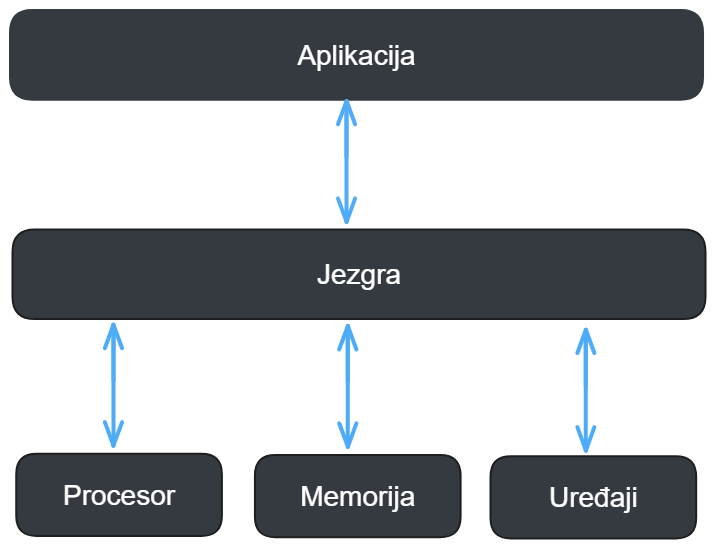
\includegraphics[width=0.7\textwidth]{slike/Grada_racunala.png}
    \caption{Građa računala (Izvor: \citeauthor{Grada})}
    \label{fig:grada}
\end{figure}

\begin{figure}[ht!]
    \centering
    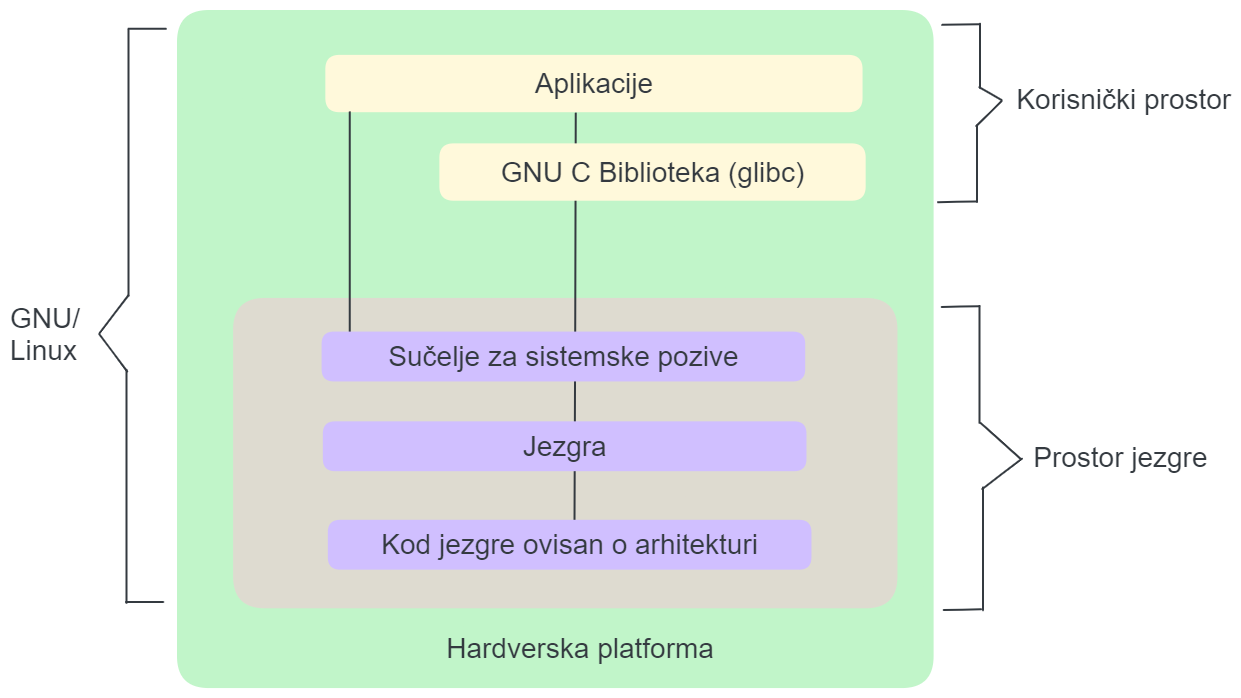
\includegraphics[width=0.9\textwidth]{slike/Arhitektura_linuxa.png}
    \caption{Arhitektura linuxa (Izvor: \citeauthor{Arhitektura})}
    \label{fig:arhitektura}
\end{figure}

GNU, punog imena GNU's Not Unix (hrv. \textit{GNU Nije Unix}) je besplatan operacijski sustav koji prati filozofiju slobodnog softvera (engl. \textit{free software}) koja se u određenoj mjeri razlikuje od filozofije otvorenog koda (engl. \textit{open source}). Projekt razvijanja GNU sustava naziva se GNU Project, a nastao je 1983. godine kada je većina softvera bila zatvorenog koda i/ili pod komercijalnom licencom. Do 1990. godine su razvijeni svi dijelovi operacijskog sustava osim jezgre te je 1992. godine u GNU sustav integrirana Linux jezgra čime je nastao GNU/Linux operacijski sustav koji je danas poznatiji samo pod imenom Linux. (Slika \ref{fig:arhitektura}) GNU Project je također razvio grafičko radno okruženje GNOME koje se uz grafičko okruženje KDE koristi u većini GNU/Linux distribucija (engl. \textit{"distros"}).\cite{GNU} GNU/Linux sustav ima puno različitih distribucija koje su se kroz povijest granale od nekoliko glavnih distribucija, no uglavnom sve za ljusku (engl. \textit{shell}) koriste Bash skriptni jezik te stoga nije važno koja se GNU/Linux distribucija promatra u kontekstu ovog rada.

GNU/Linux operacijski sustav se koristi na 96.3\% od najkorištenijih milijun servera na svijetu.\cite{Statistika} To proizlazi iz njegove stabilnosti, sigurnosti i modela otvorenog koda. Linux jezgra je modularna, što znači da je prilikom nadogradnje nekog modula jezgre, primjerice drivera uređaja, potrebno samo ponovno pokrenuti taj modul, a ne cijeli sustav što serverima daje stabilnost i osigurava posluživanje.\cite{Modularnost} Sigurnost proizlazi iz same činjenice da su GNU/Linux distribucije najčešće otvorenog koda te je gotovo nemoguće implementirati tajni pristup (engl. \textit{back door}). Također koristi vrlo strog sustav dopuštenja korisnicima (engl. \textit{user privilege}) i sustavi za rad s paketima (engl. \textit{package management systems}) imaju implementirane provjere sigurnosti i česta provjerena ažuriranja.\cite{Sigurnost} Android operacijski sustav također koristi Linux za svoju jezgru, kao i mnogi drugi manji uređaji.

\section{Mogućnosti instalacije, WSL 2}
GNU/Linux operacijski sustav se može koristiti na više načina\cite{MS_howto}:
\begin{itemize}
    \item Virtualna mašina u oblaku (engl. \textit{cloud VM})
    \item Lokalna virtualna mašina (engl. \textit{local VM})
    \item Sustav dvostrukog pokretanja (engl. \textit{dual boot})
    \item Glavni operacijski sustav
    \item WSL 2
\end{itemize}
Za primjer jedne mogućnosti instalacije neke GNU/Linux distribucije ću proći korake instaliranja Ubuntu distribucije na sustavu WSL (engl. \textit{Windows Subsystem for Linux}). WSL je sustav, tj. sloj kompatibilnosti (engl. \textit{Compability layer}) na Windows operacijskom sustavu koji omogućuje istovremeno korištenje GNU/Linux distribucije i Windows operacijskog sustava.\cite{MS_whatis_wsl} WSL izravno podržava brojne distribucije kao što su: Ubuntu, Debian, OpenSUSE / SUSE, Kali Linux i druge. (Slika \ref{fig:distribucije}) U osnovi, WSL omogućava izolirano pokretanje i korištenje GNU/Linux distribucije sa svojim vlastitim datotečnim sustavom (engl. \textit{file system}) koji je odvojen od Windows datotečnog sustava i drugih potencijalno instaliranih distribucija. WSL 2 je druga i najnovija verzija WSL sustava koji koristi podskup Hyper-V arhitekture za virtualizaciju koja omogućava bolje performanse i integraciju.\cite{hyperv}
WSL ima vrlo jednostavnu instalaciju na Windows 10 verziji 2004 i više i Windows 11 operacijskim sustavima\cite{MS_install_wsl}. U Windows Powershell ili Naredbeni Redak (engl. \textit{Command Prompt}) u načinu rada kao administrator potrebno je upisati:

\lstdefinestyle{vece}{
    basicstyle=\ttfamily\large
}

\begin{lstlisting}[language=bash]
wsl --install
\end{lstlisting}

\begin{flushleft}i zatim ponovno pokrenuti računalo. Naredba će zadano instalirati Ubuntu distribuciju, no distribucija se može specificirati naredbom:\end{flushleft}

\begin{lstlisting}[language=bash]
wsl --install -d <Ime distribucije>
\end{lstlisting}

\begin{flushleft}gdje se izravno podržane distribucije mogu vidjeti naredbom:\end{flushleft}

\begin{lstlisting}[language=bash]
wsl --list --online
\end{lstlisting}

\begin{figure}[H]
    \centering
    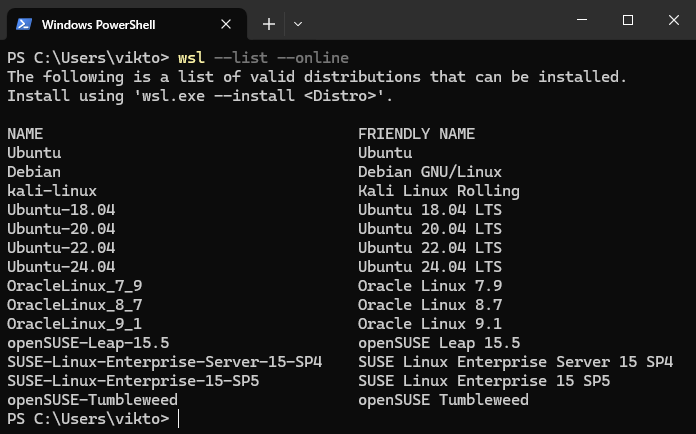
\includegraphics[width=0.9\textwidth]{slike/lista_distribucija.png}
    \caption{Izravno podržane distribucije (Izvor: autor)}
    \label{fig:distribucije}
\end{figure}

\begin{flushleft}S obzirom da za ovaj rad koristim Ubuntu distribuciju, nije potrebno specificirati distribuciju. Sada se Ubuntu distribuciji može pristupiti ili jednostavnim upisivanjem imena distribucije, u ovom slučaju \textit{ubuntu}, ili pronalaženjem instalirane distribucije u Windows Start Menu.\end{flushleft}


\chapter{Naredbeno-linijsko sučelje OS-a}

Operacijski sustavi imaju dva načina tj. sučelja preko kojih im se može pristupati. Danas je najčešće sučelje grafičko korisničko sučelje (engl. \textit{graphical user interface, GUI}), ali povijesno najkorištenije i ono koje je prisutno u svakom operacijskom sustavu je naredbeno-linijsko sučelje (engl. \textit{command line interface, CLI}). Kao što je rečeno, naredbeno-linijsko sučelje je softverski mehanizam preko kojega se uz pomoć tipkovnice može djelovati na operacijski sustav.\cite{AWSShell} Neke od prednosti naredbeno-linijskog sučelja nad grafičko korisničkog sučelja su:\cite{AWSShell}
\begin{itemize}
    \item Efikasnost
    \item Udaljeni pristup (engl. \textit{remote access})
    \item Otklanjanje poteškoća (engl. \textit{troubleshooting})
\end{itemize}
Efikasnost korištenja naredbeno-linijskog sučelja proizlazi iz toga što se jednom naredbom može djelovati na više datoteka, može se uspostaviti cjevovod naredbi (engl. \textit{command pipeline}) koji će kasnije u radu biti detaljnije objašnjen, mogu se stvoriti skripte za automatiziranu radnju nekih rutinskih i učestalih poslova što će također biti pomno objašnjeno i činjenica da iskusni korisnici mogu brže obavljati radnje nego preko grafičkog sučelja. Naredbeno-linijsko sučelje je u većini slučajeva jedini način za udaljeni pristup uređajima poput servera ili drugih fizički udaljenih uređaja iz razloga što takvi uređaji nemaju razloga imati grafičko sučelje jer bi to samo povećavalo korištenje resursa i potrošnju sustava. Otklanjanje poteškoća je u kompleksnim situacijama lakše za odraditi preko naredbeno-linijskog sučelja iz razloga što se može brže i efikasnije pristupiti, filtrirati i čitati sistemski dnevnik (engl. \textit{sistem log}) i dnevnik pogrešaka (engl. \textit{error log}), ali i iz razloga što je dokumentacija naredbi i pogrešaka u naredbeno-linijskom sučelju vrlo dobro i opsežno dokumentirana.\cite{AWSShell}

Kao što je rečeno, naredbeno-linijsko sučelje je softverski mehanizam, a konkretna implementacija naredbeno-linijskog sučelja se zove ljuska (engl. \textit{shell}). Ljuska je program koji prima naredbe preko tipkovnice i daje ih operacijskom sustavu na izvršavanje.\cite{LinuxCommand} Postoje razne ljuske, primjerice bash na GNU/Linux ili cmd.exe i PowerShell na Windows operacijskom sustavu.\cite{AWSShell} U početnim danima Unix sustava se koristio višekorisnički (engl. \textit{multi-user}) sustav na glavnom (engl. \textit{mainframe}) računalu gdje bi se korisnici udaljenim pristupom spajali na glavno računalo preko individualnih terminala koji su samo tipkovnica i ekran bez dovoljno snage da lokalno pokreću programe. Preko terminala bi se uneseni znakovi slali na glavno računalo te bi se na ekran prikazivala povratna informacija od glavnog računala. Sve radnje su se radile preko svojih programa ili naredbi, primjerice za stvoriti direktorij, izlistati sadržaj, preimenovati datoteku i slično. Ti programi se nalaze u jednom glavnom programu koji ih učahuruje što je u stvari ljuska.\cite{UbuntuShell} Originalnu Unix ljusku \textit{The Bourne \textbf{Sh}ell}, sh, je razvio Stephen Bourne dok je bio zaposlen u Bell Labs, a 1979. godine ju je izdao u Unix verziji 7 koja je bila distribuirana fakultetima i sveučilištima. Bash ljuska, punog imena \textit{\textbf{B}ourne \textbf{A}gain \textbf{Sh}ell}, je besplatna zamjena otvorenog koda za originalni \textit{Bourne Shell} i zbog svoje prirode otvorenog koda je zadana ljuska na GNU/Linux sustavima.\cite{ShellHistory}
\begin{flushleft}
    Iako je terminal u povijesti bilo ime za fizički uređaj preko kojega se spajalo na glavno računalo, danas se također koristi terminal no u drugačijoj implementaciji. Terminal (engl. \textit{terminal emulator}) je program koji otvara prozor preko kojega se komunicira sa ljuskom.\cite{LinuxCommand} Da sumiram, preko terminala se komunicira sa ljuskom koja je konkretna implementacija naredbeno-linijskog sučelja. Koraci koji se odvijaju nakon što se upiše naredba u naredbeno-linijsko sučelje neovisno u ljusci su sljedeći\cite{AWSShell}:
\begin{itemize}
    \item interpretator naredbenog retka (engl. \textit{CLI interpreter}) ljuske raščlanjuje (engl. \textit{parse}) naredbu kako bi dobio njenu strukturu i sve naredbe, opcije i argumente
    \item ljuska pregledava nazive naredbi u listi
    \item ljuska pretražuje \textit{PATH} varijablu sustava što je lista direktorija gdje se datoteke na sustavu nalaze kako bi pronašla datoteke koje su asocirane sa naredbom
    \item ljuska poziva datoteke i prosljeđuje im opcije i argumente
    \item operacijski sustav obavi radnju koja je zadana naredbom
    \item vraća se povratna vrijednost u obliku rezultata operacije, poruke pogreške, podataka ili drugo
    \item ljuska prikazuje povratnu informaciju na ekran
\end{itemize}
\end{flushleft}

\section{Osnove GNU/Linux naredbenog sučelja}
\begin{figure}[H]
    \centering
    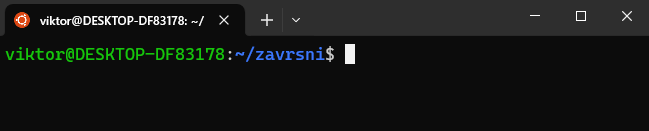
\includegraphics[width=0.9\textwidth]{slike/terminal.png}
    \caption{Prazan terminal (Izvor: autor)}
    \label{fig:terminal}
\end{figure}
Slika \ref{fig:terminal}. prikazuje prazan terminal nakon što se uđe u Ubuntu distribuciju. Sintaksa upita (engl. \textit{prompt}) je sljedeća:

\begin{lstlisting}[language=bash]
korisnickoime@nazivracunala:lokacija$
\end{lstlisting}

\begin{itemize}
    \item korisnickoime (viktor) -> označava korisničko ime trenutno prijavljenog korisnika
    \item nazivracunala (DESKTOP-DF83178) -> označava ime sistema na kojega smo prijavljeni
    \item lokacija (\textasciitilde{}/zavrsni) -> putanja lokacije na kojoj se nalazimo
    \item \$ -> simbol upita (engl. \textit{prompt symbol}) koji označava vrste prava korisnika. \$ označava standardna prava, dok \# označava administratorska prava (engl. \textit{root privileges})
\end{itemize}

\begin{flushleft}
Svaka naredba prati sljedeću standardnu sintaksu:
\end{flushleft}

\begin{lstlisting}[language=bash]
naredba [-argument] [--puni naziv argumenta] datoteka
\end{lstlisting}

\begin{flushleft}
Primjer dugačkog tj. punog naziva argumenta je -{}-long, a skraćeni naziv tog argumenta je -l. Skraćeni nazivi argumenata se mogu spajati pa umjesto pisanja argumenata -l -a je moguće napisati -la. Važno je napomenuti da su bash ljuska i GNU/Linux datotečni sustav osjetljivi na kapitalizaciju slova (engl. \textit{case sensitive}) te su stoga Datoteka.txt i datoteka.txt dvije različite datoteke kao što su pwd i PWD dvije različite, tj. jedna postojeća jedna nepostojeća naredba. Također je važno napomenuti da nije potrebno pisati tip datoteke (primjerice .exe) jer se ona automatski iščitava od strane operacijskog sustava.
\end{flushleft}

\subsection{Navigacija}
Najvažnije naredbe za navigaciju kroz datotečni sustav su:
\begin{itemize}
    \item \verb|pwd| (engl. \textit{print working directory}) prikazuje apsolutnu putanju od korijenskog direktorija '/' do direktorija u kojemu se korisnik nalazi kada ju izvrši, tj. radnog direktorija. (Slika \ref{fig:pwd})
    \item \verb|cd| (engl. \textit{change directory}) prima argument putanje do direktorija u kojega se korisnik želi prebaciti. Za putanju direktorija se uvijek može koristiti ili apsolutna ili relativna putanja, tj. putanja od korijenskog direktorija ili putanja od radnog direktorija. Ako se korisnik želi prebaciti u direktorij koji prethodi trenutnom, može koristiti argument \verb|..| umjesto putanje. (Slika \ref{fig:cd})
    \item \verb|clear|, \verb|history| iako ne spadaju u naredbe za navigaciju, napomenuti ću ih na početku jer su vrlo korisne naredbe koje će se često koristiti kroz ikakav rad s ljuskom. Naredba \verb|clear| naizgled briše sav prethodan sadržaj sa terminala no zapravo ga pomiče prema gore gdje nije vidljiv u terminalu. Naredba \verb|history| izlistava povijest svih prethodno izvršenih naredbi u ljusci.
\end{itemize}

\begin{figure}[H]
    \centering
    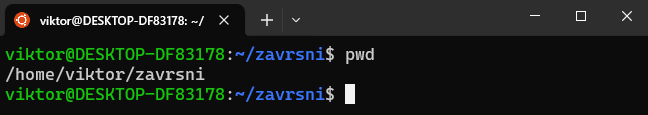
\includegraphics[width=0.9\textwidth]{slike/pwd.png}
    \caption{Naredba pwd (Izvor: autor)}
    \label{fig:pwd}
\end{figure}
\begin{figure}[h!]
    \centering
    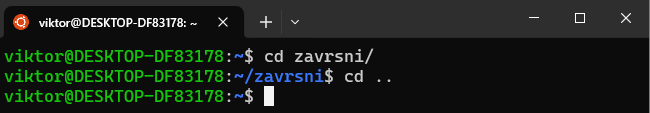
\includegraphics[width=0.9\textwidth]{slike/cd.png}
    \caption{Naredba cd (Izvor: autor)}
    \label{fig:cd}
\end{figure}

\subsection{Pregledavanje}
Najvažnije naredbe za pregledavanje datoteka su:
\begin{itemize}
    \item \verb|ls| (engl. \textit{list} izlistava sadržaj direktorija u kojemu se korisnik nalazi. (Slika \ref{fig:ls}) \verb|ls| može primiti velik broj argumenata, no najvažniji su: \verb|-a|, \verb|-l|, \verb|-h| i \verb|-d|. Argument \verb|-a| izlistava sav sadržaj direktorija uključujući i inače sakrivene datoteke koje počinju s točkom. Argument \verb|-l| prikazuje dugačak format liste gdje je prikazano: dopuštenja (engl. \textit{permissions}), vlasnik, grupa, veličina, datum izmjene i naziv. Argument \verb|-h| zajedno s prethodnim argumentom veličinu datoteke prikazuje u čitljivijem formatu. Zadnji je argument \verb|-d| koji izlistava samo direktorije.
    \item \verb|less| je jednostavan program za pregledavanje tekstualnog sadržaja. Omogućava pregledavanje tekstualne datoteke po stranicama i pretraživanje teksta unutar datoteke. Prednost ovog programa je što ne učitava cijeli sadržaj tekstualne datoteke pri otvaranju što ga čini vrlo efikasnim pri radom sa velikim tekstualnim datotekama. Korisno je napomenuti da se iz programa izlazi tipkom 'q'.
    \item \verb|cat| služi za pregledavanje sadržaja tekstualne datoteke, no za razliku od \verb|less| sadržaj datoteke ispisuje na ekran terminala. Njena sintaksa je \verb|cat ime_datoteke|
    \item \verb|file| je naredba koja određuje tip datoteke na temelju sadržaja što je korisno kada vrsta datoteke nije jasna prema ekstenziji ili nazivu. (Slika \ref{fig:ls})
\end{itemize}
\begin{figure}[H]
    \centering
    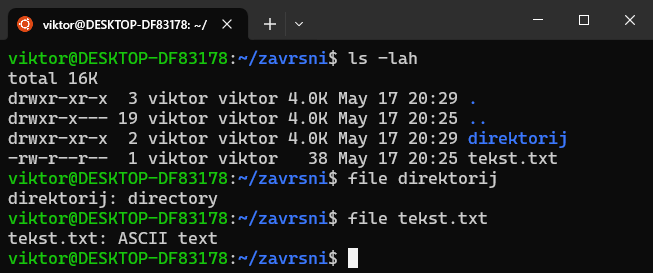
\includegraphics[width=0.9\textwidth]{slike/ls_file.png}
    \caption{Naredbe ls i file (Izvor: autor)}
    \label{fig:ls}
\end{figure}

\subsection{Manipuliranje}
Najvažnije naredbe za manipuliranje datoteka su:
\begin{itemize}
    \item \verb|cp| (engl. \textit{copy}) je naredba koja se koristi za kopiranje datoteka i direktorija. Sintaksa naredbe je sljedeća: \verb|cp izvorište odredište|. Primjer naredbe koja će kopirati tekstualnu datoteku 'datoteka.txt' u direktorij 'direktorij' je: \verb|cp datoteka.txt direktorij/|
    \item \verb|mv| (engl. \textit{move}) je naredba koja se koristi za premještanje i/ili preimenovanje datoteka i direktorija. Sintaksa naredbe je ista kao i kod prethodno naredbe: \verb|mv izvorište odredište|, no razlika je što ako želimo primjerice preimenovati datoteku 'tekst' u 'tekst1' tada će naredba glasiti ovako: \verb|mv tekst.txt tekst1.txt|
    \item \verb|rm| (engl. \textit{remove}) je naredba koja se koristi za brisanje datoteka i direktorija. Njena sintaksa je: \verb|rm [opcije] datoteke|. Najčešće korišteni argumenti su \verb|-r| koji označava rekurzivno brisanje direktorija i njihovih sadržaja i \verb|-v| koji omogućuje detaljno ispisivanje informacija o sadržaju koji se briše. U sljedećem se primjeru u direktoriju 'za\_brisanje' nalaze dvije tekstualne datoteke 'tekst1' i 'tekst2'. Korištenjem \verb|rm -rv za_brisanje| se briše i direktorij i njegove datoteke i ispisuje se što se obrisalo (Slika \ref{fig:rm}).
    \item \verb|mkdir| je naredba koja služi za kreiranje direktorija. Njena sintaksa je: \verb|mkdir ime_direktorija|.
    \item \verb|nano| je jednostavan program za uređivanje tekstualnih datoteka koji omogućava stvaranje i uređivanje tekstualnih datoteka. Njegova sintaksa je: \verb|nano ime_datoteke|
\end{itemize}
\begin{figure}[H]
    \centering
    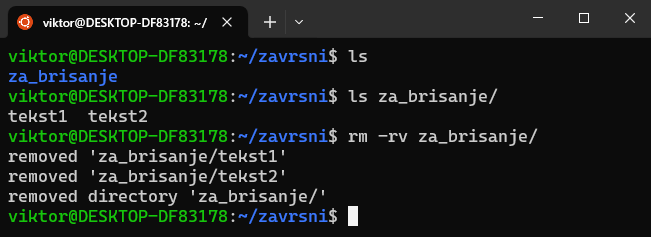
\includegraphics[width=0.9\textwidth]{slike/rm.png}
    \caption{Naredba rm (Izvor: autor)}
    \label{fig:rm}
\end{figure}

\subsection{Upute}
Najvažnije naredbe za dobivanje uputa i informacija su:
\begin{itemize}
    \item \verb|help| i \verb|man| (engl. \textit{manual}) su naredbe kojima se može pročitati dokumentacija za naredbe i funkcije. Naredba \verb|help| prikazuje informacije samo o naredbama ljuske. Naredba \verb|man| prikazuje dokumentaciju o bilo kojem programu ili naredbi za koju postoji priručnik u sustavu. Sintakse su: \verb|help naredba| i \verb|man naredba|
    \item \verb|type| je naredba koja prikazuje informacije, tj. kako je naredba definirana i gdje se nalazi, o tipu naredbe ili funkcije. Sintaksa je: \verb|type naredba|
    \item \verb|which| je naredba koja prikazuje lokaciju izvršne datoteke koja je dana kao argument. Naredba \verb|which| za tu informaciju pretražuje prethodno spomenutu '\textit{PATH}' varijablu.
\end{itemize}

\subsection{Preusmjeravanje ulaza/izlaza, cjevovod, filter}
Naredbe poput \verb|ls| ispisuju svoj izlazni sadržaj (engl. \textit{output}) na ekran, ali taj izlaz se može preusmjeriti korištenjem preusmjeravanja ulaza/izlaza (engl. \textit{I/O redirection}). Naredba svoj izlazni sadržaj šalje na standardni izlaz (engl. \textit{standard output}), ali simbolom '>' se izlaz naredbe može preusmjeriti na datoteku, uređaj ili ulaz druge naredbe. Ako želimo preusmjeriti izlaz naredbe \verb|ls| u tekstualnu datoteku, naredba bi glasila \verb|ls > tekst.txt|. Ako želimo da se izlaz samo pridoda sadržaju postojeće datoteke, koristimo simbol '>>'. Naredbe svoj ulaz primaju iz standardnog ulaza (engl. \textit{standard input}) koji je po zadanom načinu rada tipkovnica, ali se također može preusmjeriti sa '<'. Tako bi primjerice tekstualnu datoteku mogli sortirati tako što naredbi za sortiranje kao ulaz zadamo tekstualnu datoteku: \verb|sort < tekst.txt|. Naredba \verb|sort| za standardni izlaz ima ekran, pa se izlaz može također preusmjeriti: \verb|sort < tekst.txt > sortirano.txt|. Ovime ulazimo u tehniku cjevovoda (engl. \textit{pipeline}) gdje je izlaz jedne naredbe ulaz druge.\cite{LinuxCommandIO}
Primjer cjevovoda je \verb+ls -l | less+ gdje se izlaz \verb|ls -l| naredbe otvara u programu \verb|less|. Prilikom korištenja cjevovoda se najčešće koriste filter naredbe poput:
\begin{itemize}
    \item \verb|sort| je naredba koja sortira dani ulaz. Naredba prima opcije argumente poput \verb|-r| što označava sortiranje silaznim poretkom.
    \item \verb|uniq| (engl. \textit{unique}) je naredba koja eliminira duplikate iz ulaza i ostavlja samo jedinstvene ulaze.
    \item \verb|grep| (engl. \textit{global regular expression print}) je naredba koja pretražuje ulaz za dani uzorak. Sintaksa naredbe je: \verb|grep [opcije] uzorak [ulaz]|, primjerice \texttt{grep -i a* tekst.txt} će pretražiti datoteku tekst.txt za sve linije koje sadrže veliko ili malo slovo 'a' na početku.
    \item \verb|head| je naredba koja po zadanom načinu rada ispisuje prvih 10 linija ulazne datoteke. Ako se želi promijeniti broj prikazanij linija, to se čini sa 'n' argumentom: \texttt{head -n 5 tekst.txt}
    \item \verb|tail| je naredba slična prethodnoj naredbi samo što ispisuje zadnjih 10 ulaza, a sintaksa je identična \verb|head| naredbi.
\end{itemize}
\begin{flushleft}
    Sada kada su objašnjeni filteri, primjer korisnog cjevovoda koji bi se koristio u svakodnevnim situacijama kod obrade tekstualnih sadržaja je kada korisnik želi iz ne sortiranog teksta sa dupliciranim linijama dobiti sortirani sadržaj bez duplikata. To se može postići cjevovodom \verb+cat nesortirani_duplikati.txt | sort | uniq+ gdje se \verb|cat| koristi za otvaranje sadržaja datoteke i prenošenjem izlaza u \verb|sort| koji zatim sortirani izlaz prenosi u \verb|uniq| koji na svoj standardni izlaz koji je ekran ispisuje jedinstveni dobiveni tekstualni sadržaj. (Slika \ref{fig:cjevovod}) Važno je napomenuti da cjevovod djeluje samo u radnoj memoriji računala te primijenjene naredbe ne djeluju na samu datoteku ako se to izravno ne specificira sa preusmjeravanjem izlaza u tu datoteku\cite{UbuntuPipeline}.
\end{flushleft}
\begin{figure}[H]
    \centering
    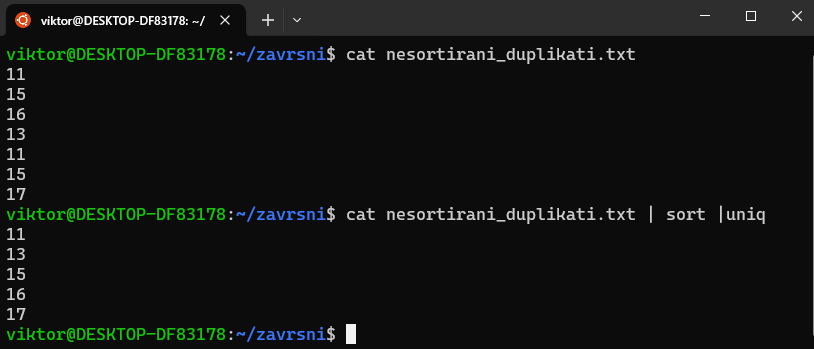
\includegraphics[width=0.9\textwidth]{slike/cjevovod.png}
    \caption{Primjer cjevovoda (Izvor: autor)}
    \label{fig:cjevovod}
\end{figure}

\subsection{Proširenje}
Proširenje (engl. \textit{expansion} je mehanizam ljuske koji omogućuje se ono što napišemo proširi u nešto drugo prije nego ljuska obradi naredbu\cite{LinuxCommandExpansion}. Primjer je '*' koji je zamjenski znak (engl. \textit{wildcard}) za bilo koji drugi znak\cite{LinuxCommandPermissions}.
Naredba \verb|echo| je jednostavna naredba koja ispisuje tekstualni argument na standardni izlaz. Ako se izvrši \verb|echo Ovo je test| izlaz će biti "Ovo je test". No ako se izvrši \verb|echo *| izlaz je sljedeći (Slika \ref{fig:echo}):

\begin{figure}[H]
    \centering
    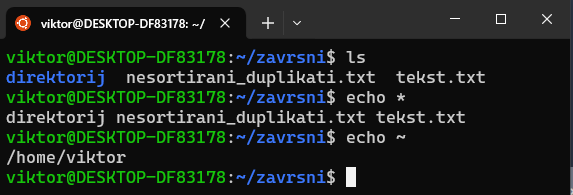
\includegraphics[width=0.9\textwidth]{slike/echo.png}
    \caption{Proširivanje sa naredbom echo (Izvor: autor)}
    \label{fig:echo}
\end{figure}

\begin{flushleft}
Naredba \verb|echo| je ispisala sadržaj radnog direktorija. To je zato što prije nego što se naredba izvršila, ljuska je proširila argument '*' u sve kvalificirajuće argumente, što je u ovom slučaju sadržaj direktorija, i time je naredba kao ulaz dobila rezultat tog proširenja, a ne znak '*'. Proširenje se također vrši nad znakom '\textasciitilde{}' kojeg ljuska proširuje u ime 'home' direktorija korisnika. (Slika \ref{fig:echo})
\end{flushleft}
\begin{flushleft}
Proširenje se koristi i za obavljanje računanja tj. aritmetike u ljusci.\cite{LinuxCommandExpansion}). Sintaksa \verb|$((izraz))| omogućava obavljanje matematičkih operacija nad cijelim brojeva u ljusci. Primjerice, \verb|echo $((1+1))| na terminal ispisuje '2'. Može se koristiti i ugnježđivanje poput \verb|echo (((5**2)*3))| što na terminal ispisuje '75'. Ljuska također podržava operacije cjelobrojnog dijeljenja '\%' i dijeljenja '\textbackslash{}'.
\end{flushleft}
\begin{flushleft}
Jedna od naprednijih tehnika proširenja je proširenje zagradama (engl. \textit{brace expansion}). Proširenje zagradama od danog uzorka stvara više linija teksta što može služiti kao više argumenata koji se automatski generiraju. Primjer proširenja zagradama je naredba \verb|echo a{1,2,3}b| koja ispisuje sljedeće 'a1b a2b a3b' (Slika \ref{fig:prosirenjezagradama}). Umjesto pojedinih znakova se može zadati i raspon poput \verb|echo {1..5}| ili \verb|echo {A..E}|. Ova tehnika je najkorisnija kod stvaranja velikog broja datoteka ili direktorija koji slijede neki uzorak. Primjerice, ako želimo stvoriti direktorije koji prate format 'godina-mjesec' za svaki mjesec u godini 2024., naredba bi bila \verb|mkdir 2024-{01..12}| (Slika \ref{fig:prosirenjezagradama}).
\end{flushleft}
\begin{figure}[H]
    \centering
    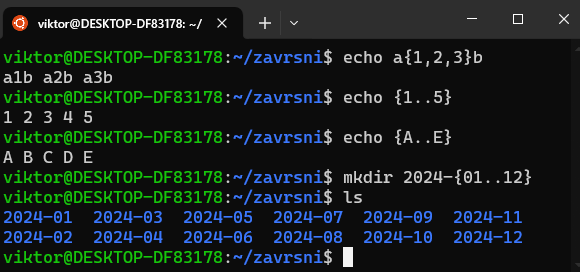
\includegraphics[width=0.9\textwidth]{slike/prosirenje.png}
    \caption{Primjeri proširenja zagradama (Izvor: autor)}
    \label{fig:prosirenjezagradama}
\end{figure}
\begin{flushleft}
Još dva koncepta koja ću ukratko objasniti no koja će biti temeljnije pojašnjena kasnije u radu su proširenje parametara (engl. \textit{parameter expansion}) i substitucija naredbi (engl. \textit{command substitution}). Proširenje parametara je mogućnost stvaranja varijabli i njihovo dodjeljivanje vrijednosti. Sam operacijski sustav ima listu varijabli koja je vidljiva sa naredbom \verb+printenv |less+, a vrijednost specifične varijable, primjerice 'USER' se može saznati sa \verb|echo $USER|. Substitucija naredbi je tehnika u kojoj se izlaz jedne naredbe koristi kao proširenje. Primjer toga je redak \verb+file $(ls /usr/bin/* | grep bin/zip*)+. Ova naredba izlaz \verb|ls| naredbe daje kao ulaz \verb|grep| naredbi koja traži sve ulazne linije koje počinju sa uzorkom znakova 'zip' te se taj finalni popis daje naredbi \verb|file| kao ulaz. (Slika \ref{fig:sub})
\end{flushleft}
\begin{figure}[H]
    \centering
    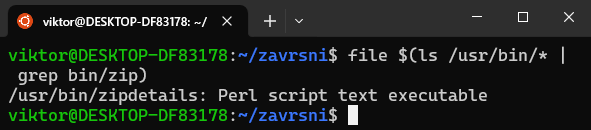
\includegraphics[width=0.9\textwidth]{slike/substitucija.png}
    \caption{Primjer substitucije naredbi (Izvor: autor)}
    \label{fig:sub}
\end{figure}

\subsection{Dopuštenja}
Sustav dopuštenja proizlazi iz činjenice da na jednoj mašini u isto vrijeme mogu raditi više korisnika korištenjem udaljenog pristupa što stvara potencijalne konflikte i probleme. Postoje tri vrste prava, 'r' (engl. \textit{read}) - pravo čitanja, 'w' (engl. \textit{write}) - pravo pisanja i 'x' (engl. \textit{execute}) - pravo izvršavanja. Svaki direktorij i datoteka imaju postavljeno svoja dopuštenja za vlasnika, grupu i ostale korisnike. Kao što je vidljivo na (Slika \ref{fig:ls}) format zapisa dopuštenja je '-rwxrwxrwx'. Prvi znak može biti '-' u slučaju da se radi o datoteci, ili 'd' ako se radi o direktoriju. Sljedeća tri znaka se odnose na dopuštenja vlasnika te datoteke, druga tri na dopuštenja grupe, a zadnja tri na dopuštenja svih ostalih korisnika.\cite{LinuxCommandPermissions}
Najvažnije naredbe za dobivanje i mijenjanje dopuštenja su:
\begin{itemize}
    \item \verb|chmod| je naredba koja služi za mijenjanje dopuštenja nad datotekom ili direktorijem. Naredba koristi oktalni sustav koji se preračunava iz binarne maske koja predstavlja svako dopuštenje. Primjerice, rwxrwxrwx se u binarnom zapisu zabilježava kao 111 111 111, rw-rw-rw- kao 110 110 110, itd. S obzirom da je binarno 001 u oktalnom sustavu 1, 010 u oktalnom sustavu 2 i 100 u oktalnom sustavu 4, 111 daje 7, 101 daje 5, itd. \verb|chmod| za svaku grupu spomenutih korisnika koristi jedan oktalni broj, primjerice ako želimo postaviti dopuštenja rw-{}-{}-{}-{}-{}-{}-, tj. da je datoteka vidljiva i pristupačna samo vlasniku datoteke, koristit će se \verb|chmod 600|. Sintaksa naredbe je \verb|chmod vrijednost datoteka|
    \item \verb|sudo| je naredba koja za izvršavanje neke druge naredbe daje administratorska prava. Njena sintaksa je \verb|sudo naredba|
    \item \verb|su| je zastarjela naredba koja pokreće novu ljusku sa administratorskim pravima. Ova naredba možda ni nije podržana u novijim distribucijama te je u praktičnom smislu zamijenjena sa \verb|sudo -i| koji obavlja istu funkcionalnost.
    \item \verb|chown| je naredba koja mijenja vlasnika neke datoteke. Njena sintaksa je \texttt{chown [opcije] korisnik[:grupa] datoteka/e} primjerice ako vlasništvo datoteke 'tekst.txt' želimo prebaciti na korisnika 'ivan' tada će naredba glasiti \verb|chown ivan tekst.txt|
\end{itemize}

\chapter{Skriptiranje u Bash ljusci}
Bash skripte su datoteke koje sadrže slijed naredbi koje se izvršavaju liniju po liniju. Bash skripte se koriste zbog\cite{freecodecamp}:
\begin{itemize}
    \item automatizacije - pomoću skripti se ponavljajuće radnje i procesi mogu automatizirati što ubrzava rad na rutinskim zadacima, omogućava brzo i efikasno dobivanje informacija i olakšava obradu podataka.
    \item portabilosti - skripte se mogu pokretati na više platformi i operacijskih sustava poput UNIX, GNU/Linux, macOS i čak Windows sustava.
    \item fleksibilnosti i pristupačnost - skripte se lagano stvaraju, uređuju i izvršavaju sa ugrađenim alatima koji su prisutni u ljusci što znači da se ne moraju instalirati dodatni programi, i mogu se kombinirati s drugim jezicima za moćnije funkcionalnosti.
    \item integracije - skripte se mogu integrirati sa bazama podataka, web serverima i slično za olakšanu administraciju sustava i praćenje.
    \item otklanjanja pogrešaka (engl. \textit{debugging}) - bash skripte imaju ugrađen sustav otklanjanja pogrešaka i informativne poruke pogreške što omogućuje lagano otklanjanje pogrešaka u skriptama.
\end{itemize}
Konvencija imenovanja upućuje da bash skripte završavaju sa ekstenzijom .sh, ali to nije obavezno. Svaka bash skripta počinje sa '\textit{shebang}' linijom koja je zapravo apsolutna putanja na bash tumač (engl. \textit{bash interpreter}) što je program koji izvršava naredbe u bash ljusci. Apsolutna putanja do bash tumača se može pronaći sa: \verb|which bash|. Uobičajeno je da je ispisana putanja \verb|/usr/bin/bash|, no '/usr/' se može izostaviti što znači da će prva linija skripte biti \verb|#!/bin/bash|. Skripti se nakon stvaranja mora dodati dopuštenje korisniku za izvršavanje što se može napraviti naredbom \verb|chmod 755 skripta.sh| ili \verb|chmod u+x skripta.sh| gdje 'u' označava trenutnog korisnika, a '+x' dodaje dopuštenje za izvršavanje.

\section{Varijable}
Varijable u bash ljusci nemaju tip podataka već mogu primiti bilo kakav ulaz. Isto kao i kod drugih jezika, varijable mogu biti globalne ili lokalne. Konvencija imenovanja nalaže da imena varijabli počinju ili slovom ili znakom '\_', da imena varijabli smiju imati samo slova, brojeve i '\_' i važno je napomenuti da su varijable osjetljive na kapitalizaciju. Također nalaže da globalne varijable trebaju biti napisane velikim slovima. Varijable vrijednost mogu poprimiti direktnim upisivanjem vrijednosti ili substitucijom naredbi:
\begin{lstlisting}[language=bash]
varijabla=vrijednost
varijabla=$varijabla
varijabla=$(naredba)
\end{lstlisting}

\section{Ulaz/Izlaz}
Varijable u skriptama mogu ulaz dobiti na četiri načina: direktnom dodjelom u skripti, unosom korisnika, kroz argument skripte ili skroz datoteku. Vrijednost možemo direktno pridodijeliti varijabli u skripti, primjerice ako želimo varijabli 'tekst' dodijeliti vrijednost 'ovo je tekst': \verb|tekst="ovo je tekst"|. Korisnik može vrijednost unijeti dinamički tijekom izvođenja skripte korištenjem naredbe \verb|read|, primjerice ako želimo korisnički unos spremiti u varijablu 'tekst' i ispisati korisnički unos, kompletna skripta bi bila:
\begin{lstlisting}[language=bash]
#!/bin/bash
echo -e "\nUnesite tekst"
read tekst
echo -e "\Uneseni tekst je: "
echo $tekst
\end{lstlisting}
\begin{flushleft}
Treći način je korištenjem argumenata koji su dani prilikom pokretanja skripte. Argumentima se pristupa simbolom '\$' i brojem argumenta kojemu želimo pristupiti, primjerice \verb|$1| za prvi dani argument. Zadnji način unošenja je preko datoteke, najčešće liniju po liniju. Skripta koja čita i ispisuje datoteku liniju po liniju bi bila:
\end{flushleft}
\begin{lstlisting}[language=bash]
#!/bin/bash
while IFS= read -r linija
do
  echo "$linija"
done < ime_datoteke.txt
\end{lstlisting}
Skripte mogu preusmjeriti svoj standardni izlaz sa prijašne spomenutim metodama, primjerice kao što je vidljivo na prethodnoj skripti vrijednosti se mogu ispisivati na ekran sa naredbom \verb|echo| te se standardni izlaz naredbe također može preusmjeriti u datoteku poput \verb|echo "tekst" > datoteka.txt|.

\section{Uvjetne izjave}
Bash koristi standardne uvjetne izjave (engl. \textit{conditional statements}) koje su: \textit{if}, \textit{if-elif-else} i \textit{case}. Primjer skripte koja koristi \textit{if-elif-else} je sljedeća:
\begin{lstlisting}[language=bash]
#!/bin/bash
echo "Unesite broj: "
read broj
if [$broj -gt 0]; then
    echo "$broj je pozitivan"
elif [$broj -lt 0]; then
    echo "$broj je negativan"
else
    echo "$broj je nula"
fi
\end{lstlisting}
U ovom primjeru se koristi test uvjeta (engl. \textit{test condition}) \verb|-gt|. Testovi uvjeta su postupci tj. parametri koji provjeravaju zadovoljava li se određeni uvjet. U ovom primjeru se koristio \verb|-gt| koji provjerava je li vrijednost prije nego veća od vrijednosti poslije njega. Svi testovi uvjeta se mogu pronaći naredbom \verb|man test|, a tablica nekih od važnijih testova uvjeta je:

\begin{table}[h!] 
    \centering
    \caption{Testovi uvjeta}
    \begin{tabularx}{0.8\textwidth}{|X|X|X|}
        \hline
         \cellcolor{gray!25} test & \cellcolor{gray!25} značenje & \cellcolor{gray!25} tip \\
        \hline
        -eq & jednako & broj \\
        \hline
        -ge & veće ili jednako & broj \\
        \hline
        -gt & veće od & broj \\
        \hline
        -le & manje ili jednako & broj \\
        \hline
        -lt & manje od & broj \\
        \hline
        -ne & nije jednako & broj \\
        \hline
        -e & istina ako datoteka postoji & datoteka \\
        \hline
        -f & istina ako datoteka postoji i običnog je tipa & datoteka \\
        \hline
        -z & istina ako je tekst prazan & tekst \\
        \hline
        -n & istina ako tekst nije prazan & tekst \\
        \hline
        == & istina ako su tekstovi jednaki & tekst \\
        \hline
        != & istina ako tekstovi nisu jednaki & tekst \\
        \hline
    \end{tabularx}
    \\[10pt]
    \caption*{(Izvor: \cite{LinuxCommandTest}, \cite{Geeks})}
    \label{tab:objekti}
\end{table}

\section{Petlje}
Bash podržava tri osnovne vrste petlji: \verb|for|, \verb|while| i \verb|until|. Petlja \verb|for| se izvršava na temelju broja ponavljanja koji su zadani, a mogu se zadati ili intervalom ili time što petlja prolazi svaki element nekog polja. Petlja \verb|while| se ponavlja dok god se ne izvrši dani uvjet. Petlja \verb|until| se ispunjava dok god je dani uvjet istinit, tj. obrnuti princip od \verb|while| petlje. Sljedeća skripta pokazuje sintaksu kroz primjer korištenja sve tri vrste petlji, a njen ispis je vidljiv na slici \ref{fig:petlje}:

\begin{lstlisting}[language=bash]
#!/bin/bash

echo "for petlja"
for i in {1..5}; do
    echo -n "$i "
done
echo

echo "for-in petlja"
brojevi=(1 2 3 4 5)
for broj in "${brojevi[@]}"; do
    echo -n "$broj "
done
echo

echo "while petlja"
brojac=1
while [ $brojac -le 5 ]; do
    echo -n "$brojac "
    ((brojac++))
done
echo

echo "until petlja"
brojac=1
until [ $brojac -gt 5 ]; do
    echo -n "$brojac "
    ((brojac++))
done
echo
\end{lstlisting}
\begin{figure}[H]
    \centering
    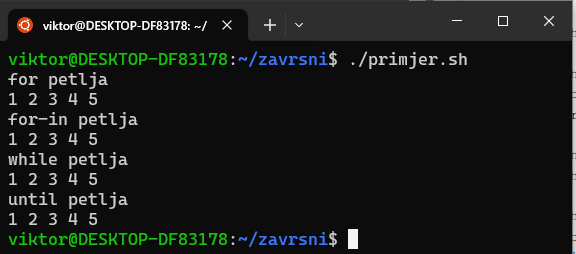
\includegraphics[width=0.9\textwidth]{slike/petlje.png}
    \caption{Ispis skripte (Izvor: autor)}
    \label{fig:petlje}
\end{figure}

\section{Ostalo}
Još ću spomenuti tri korisne stvari za bash skriptiranje, a to su \textit{cron}, \textit{otklanjanje poteškoća} i \textit{funkcije}. Cron je program koji omogućuje izvršavanje zadataka u određenim vremenskim intervalima te se može koristiti kako bi se postavilo izvršavanje skripte na neke ponavljajuće vremenske intervale poput svaki dan u točno vrijeme, svakih sat vremena, svaki prvi dan u mjesecu itd. Cron također zapisuje svoje djelovanje u dnevnik koji se nalazi na putanju '/var/log/syslog' što je korisno za praćenje eventualnih poteškoća. Otklanjanje poteškoća je ugrađena mogućnost u bash ljusku, a u skripti se može ukljućiti sa linijom \verb|set -x| koja postavlja način rada za otklanjanje poteškoća time što se ispisuje vrijednost za svaku izvršenu liniju u skripti što je istaknuto simbolom '+' prije svake linije skripte. Zadnje, bash podržava funkcije što pomaže pri preglednosti koda i ponovnoj iskoristivnosti elemenata skripti, primjer funkcija će biti pokazan kasnije u radu.

\section{Primjer}
Kao praktičan primjer Bash skriptiranja ću obraditi sljedeći scenarij. Serveri imaju svoj dnevnik u kojega se zapisuju zahtjevi napravljeni prema serveru i odgovor servera. Poželjno bi bilo imati dvije stvari: praćenje određenih tipova odgovora servera poput "401" odgovora pogreške ili drugih sličnih odgovora kada nešto nije izvedeno kako je trebalo biti i dobivanje pregleda svih takvih odgovora od zadnjeg trenutka kada smo ih pregledali, tipa ako ujutro želimo pregledati što se događalo preko noći. Za ovaj primjer sam napravio dvije Bash skripte, jedna koja simulira server koji sprema vrste odgovora u dnevnik, a druga koja u stvarnom vremenu obaviještava kada se određene poruke spreme u dnevnik i koja može dati sve poruke neke vrste od zadnjeg trenutka gledanja. Prva skripta je jednostavna jer na pojednostavljen način simulira spremanje odgovora servera. Linija \textbf{1} je prethodno spomenuti \textit{shebang} što je putanja do 
bash tumača. Linija \textbf{3} je varijabla u koju se sprema željeno ime datoteke. Linija \textbf{5} je funkcija u kojoj se u liniji \textbf{6} stvara polje sa mogućim vrstama poruka, u liniji \textbf{7} sprema jedna vrsta dobivena nasumičnim odabirom indeksa koristeći \verb|$RANDOM| globalnu varijablu, u liniji \textbf{8} generira poruka koja će se spremiti u dnevnik i u liniji \textbf{9} preusmjerava izlaz \verb|echo| naredbe koja ispisuje stvorenu poruku koja se sastoji od trenutnog datuma i vremena proizvoljnog formata, vrste odgovora i same poruke u datoteku dnevnika. Linija \textbf{12} je početak beskonačne petlje koja poziva funkciju i zatim "spava" na nasumični broj sekundi između 1 i 5.

\begin{lstlisting}[language=bash]
1 #!/bin/bash
2
3 log="server.log"
4
5    generiraj() {
6        local vrste=("INFO" "WARN" "ERROR")
7        local vrsta=${vrste[$RANDOM % ${#vrste[@]}]}
8        local poruka="Poruka tipa: $vrsta"
9        echo "$(date +'%Y-%m-%d %H:%M:%S') $vrsta: $poruka" >> $log
10    }
11
12 while true; do
13    generiraj
14    sleep $((RANDOM % 5 + 1))
15 done
\end{lstlisting}

Druga skripta analizira dnevnik i ispisuje "WARN" i "ERROR" poruke koje prva skripta zabilježi. Linija \textbf{1} je kao i uvijek \textit{shebang}, linije \textbf{3} i \textbf{4} su varijable u koje se sprema ime dnevnika i ime datoteke koja će se koristiti kao posredna datoteka u koju će se bilježiti broj "obrađenih" zapisa. Linije \textbf{6}, \textbf{7} i \textbf{8} u varijable spremaju ANSI \textit{escape code} koji se može koristiti za određivanje boje znakova u terminalu. Linija \textbf{10} je glavna funkcija u kojoj se u liniji \textbf{11} inicijalizira varijabla za zadnju poziciju koja je obrađena, linija \textbf{12} provjerava postoji li posredna datoteka čiji je naziv spremljen u \verb|$temp| varijablu, ako postoji onda kao zadnju poziciju postavlja broj iz datoteke.
Linija {16} inicijalizira broj redaka u dnevniku na 0, linija \textbf{17} provjerava postoji li dnevnik, a ako postoji onda sprema broj redaka dnevnika u varijablu. Linija \textbf{21} uspoređuje broj linija u dnevniku sa brojem zadnje obrađene linije u posrednoj datoteci, ovo je napravljeno u slučaju da se dnevnik isprazni pa je zabilježeni broj zadnje linije u posrednoj datoteci netočan. Ako je tako, \verb|zadnja_pozicija| se postavlja na 0 jer se promjena dnevnika morala dogoditi dok skripta nije bila pokrenuta. Linija \textbf{25} u varijablu \verb|novo| sprema sve linije iz dnevnika nakon zadnje linije koja je brojčano zapisana u posrednoj datoteci. Linija \textbf{27} provjerava sadrži li varijabla novo tekst, ako sadrži onda linija \textbf{28} svaku liniju sprema u varijablu \verb|linija| koju se provjerava sadrži li igdje tekst "WARN" ili "ERROR", ako sadrži na ekran se ispisuje linija u žutoj ili crvenoj boji, ovisno o vrsti poruke. Linija \textbf{37} u posrednu datoteku zapisuje novi broj zapisa dnevnika. Linija \textbf{42} određuje da skripta pokreće funkciju svaku sekundu.

\begin{lstlisting}[language=bash]
1  #!/bin/bash
2  
3  log="server.log"
4  temp=".temp_datoteka"
5  
6  CRVENA='\033[0;31m'
7  ZUTA='\033[0;33m'
8  BIJELA='\033[0m'
9  
10 analiziraj() {
11     local zadnja_pozicija=0
12     if [[ -f $temp ]]; then
13         zadnja_pozicija=$(cat $temp)
14     fi
15 
16     local broj_linija_log=0
17     if [[ -f $log ]]; then
18         broj_linija_log=$(wc -l < $log)
19     fi
20 
21     if (( broj_linija_log < zadnja_pozicija )); then
22         zadnja_pozicija=0
23     fi
24 
25     local novo=$(tail -n +$((zadnja_pozicija + 1)) $log)
26 
27     if [[ -n "$novo" ]]; then
28         echo "$novo" | while read -r linija; do
29             if [[ "$linija" == *"WARN"* ]]; then
30                 echo -e "${ZUTA}$linija$"
31             elif [[ "$linija" == *"ERROR"* ]]; then
32                 echo -e "${CRVENA}$linija$"
33             fi
34         done
35     fi
36 
37     wc -l < $log > $temp
38 }
39 
40 while true; do
41     analiziraj
42     sleep 1
43 done
\end{lstlisting}

\begin{figure}[H]
    \centering
    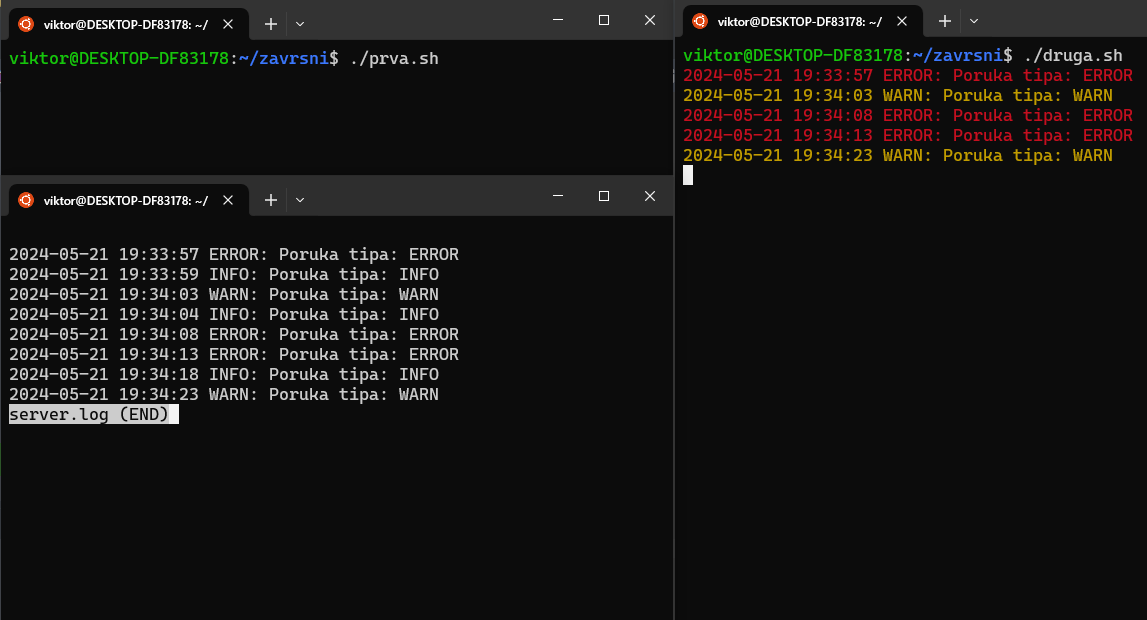
\includegraphics[width=1\textwidth]{slike/PrimjerBash.png}
    \caption{Rad skripti (Izvor: autor)}
    \label{fig:primjerbash}
\end{figure}

\chapter{.NET}

.NET je besplatna, višeplatformska (engl. \textit{cross-platform}) platforma otvorenog koda za razvijanje aplikacija koju je napravio i koju održava Microsoft. .NET se sastoji od sljedećih komponenti\cite{NETintro}:
\begin{itemize}
    \item izvršno okruženje (engl. \textit{runtime environment}) - izvršava kod aplikacije
    \item kompilator (engl. \textit{compiler}) - prevodi izvorni kod u izvršni kod za vrijeme izvođenja (engl. \textit{runtime executable code})
    \item biblioteke - sadrže unaprijed izgrađene funkcionalnosti
    \item SDK (engl. \textit{software development kit}) - komplet za razvoj softvera, tj. zbirka alatama, biblioteka i dokumentacije
    \item Skup tehnologija za razvoj aplikacija (engl. \textit{app stack}) - tehnologije za pisanje aplikacija
\end{itemize}

\begin{flushleft}
\textit{Common Language Infrastructure} (\textbf{CLI}) je "jezgra" .NET platforme i definira set pravila i specifikacija za izvršavanje .NET aplikacija time što definira formate datoteka za .NET aplikacije, specificira mehanizme za upravljanje memorijom i izvršavanje koda i standardizira sustave tipova.
\end{flushleft}

\begin{flushleft}
\textit{Common Language Runtime} (\textbf{CLR}) je virtualni stroj koji izvršava izvorni kod time što dinamički učitava i izvršava .NET kod, upravlja memorijom i upravljanjem smećem (engl. \textit{garbage collection}) i provjerava tipove.\cite{GeeksNET}
\end{flushleft}

\begin{flushleft}
\textit{Common Intermediate Language} (\textbf{CIL}) je jezik, tj. format koda koji se generira iz izvornog koda pomoću kompilatora i koji CLR može izvršavati. CIL je nezavisan o jeziku i omogućuje prenosivost koda između različitih .NET implementacija o kojima će biti riječ kasnije.
\end{flushleft}

\begin{flushleft}
\textit{Just-In-Time} (\textbf{JIT}) kompilator dinamički prevodi CIL kod u strojni kod specifičan za platformu.\cite{NETjit}
\end{flushleft}

\begin{flushleft}
\textit{Base Class Library} (\textbf{BCL}) je kolekcija ponovno iskoristivih, objektno orijentiranih klasa i metoda koje su pružaju temeljne elemente .NET aplikacija. Ove biblioteke nude sve potrebne funkcionalnosti primjerice rad s datotekama, mrežna komunikacija, kolekcija podataka i slično. BCL je usporediv "header" daototekama u C/C++ jezicima ili paketima u Java jeziku. Ovisno o .NET implementaciji ova komponenta se nekada naziva i \textit{Framework Class Library} (\textbf{FCL})\cite{GeeksNET}. Važno je i napomenuti da .NET ima svoj upravitelj paketima zvan \textit{NuGet} s kojim se mogu instalirati dodatne biblioteke napravljene od strane zajednice ili Microsoft-a.
\end{flushleft}

\begin{figure}[H]
    \centering
    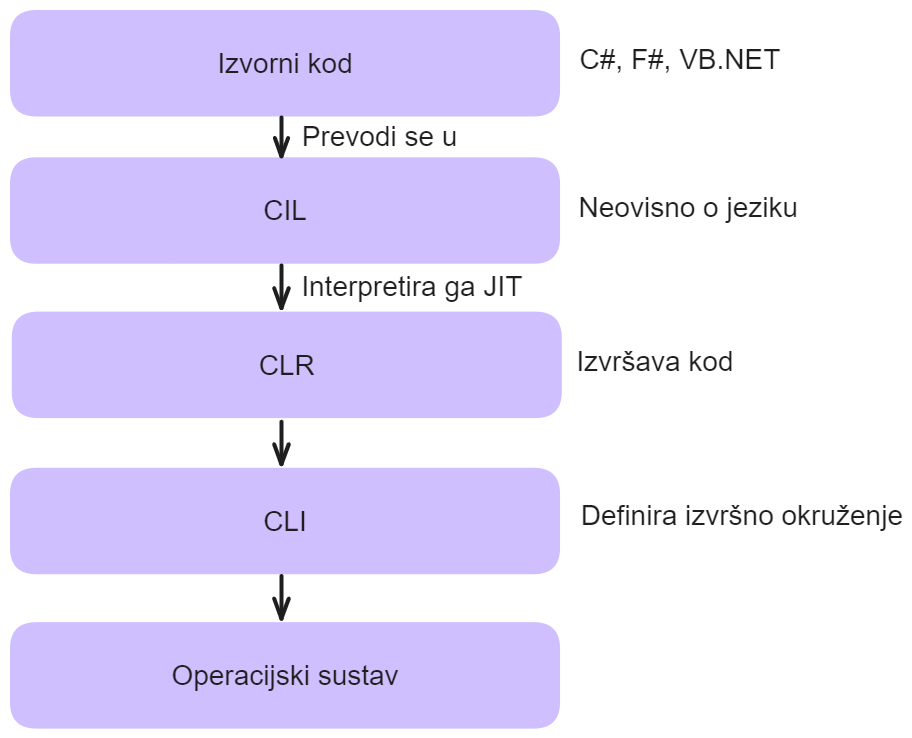
\includegraphics[width=0.7\textwidth]{slike/KomponenteNET.png}
    \caption{Pojednostavljen prikaz .NET komponenti (Izvor: autor)}
    \label{fig:netkomponente}
\end{figure}
\begin{flushleft}
Postoji više implementacija .NET-a, svaka sa svojim karakteristikama\cite{NETintro}:
\end{flushleft}
\begin{itemize}
    \item .NET Framework - originalna .NET implementacija za Windows operacijski sustav i Windows Server platformu. 
    \item .NET (Core) - preimenovano u .NET, ovo je moderna .NET implementacija koja je u potpunosti kompatibilna sa .NET Framework implementacijom ali se razlikuje po svojoj interoperabilnosti između operacijskih sustava i fokusom na \textit{cloud} aplikacije.
    \item Mono - implementacija koja je nastala od zajednice, podržana je za Android i iOS sustave.
\end{itemize}

\begin{flushleft}
Sa .NET-om se mogu razvijati\cite{sharpcorner}:
\end{flushleft}
\begin{itemize}
    \item stolne aplikacije - .NET pruža tehnologije WPF, Windows Forms, UWP i Xamarin za izgradnju stolnih aplikacija.
    \item web aplikacije - ASP.NET je skup biblioteka i alata za izgradnju web aplikacija i Blazor za izgranju jednostraničnih (engl. \textit{single-page}) web aplikacija.
    \item mobilne aplikacije - MAUI služi kao okvir za razvijanje mobilnih aplikacija sa C\# jezikom.
    \item aplikacije u oblaku - omogućuje izgradnju aplikacija za oblak koje se karakteriziraju visokom skalabilnošću, automatizacijom i visokim performansama.
    \item igrice - Unity podržava C\# i .NET tehnologije i odlično je integriran u Visual Studio.
    \item internet stvari (engl. \textit{Internet of Things - IoT})
\end{itemize}
Sada kada je jasno što je .NET kao platforma i što se s njome može, potrebno je još spomenuti podržane jezike. Izravno podržani .NET jezici su: C\#, F\# i VB.NET. To znači da neovisno u kojem jeziku pišemo svoju aplikaciju, ona će se prevesti u zajednički CIL jezik i jednako pokretati na svim sustavima i platformama zbog korištenja univerzalnih .NET elemenata koji dolaze sa .NET bibliotekama.

\section{Instalacija na GNU/Linux operacijskom sustavu}
Instalacija .NET-a se razlikuje ovisno o korištenoj distribuciji i verziji distribucije. Microsoft pruža detaljne upute za različite načine instalacije ovisno o distribuciji i verziji na svojim stranicama, no ja ću proći instalaciju za Ubuntu verziju 22.04.4 koja vrijedi i za sve verzije nakon ove, ali većim dijelom i za starije verzije. U radu će se koristiti .NET 8. Prvo je potrebno ažurirati sve pakete kako bi se prepoznala mogućnost instaliranja .NET verzije 8 te zatim instalirati SDK\cite{netinstall}:

\begin{lstlisting}[language=bash]
sudo apt-get update
sudo apt-get install -y dotnet-sdk-8.0
\end{lstlisting}
Instalaciju možemo provjeriti sa naredbom \verb|dotnet --info| koja će nam izlistati sve informacije o onome što imamo instalirano kao što su verzija .NET-a, putanje izvršnog okruđenja, putanja SDK-a i ostalo (Slika \ref{fig:info}):

\begin{figure}[H]
    \centering
    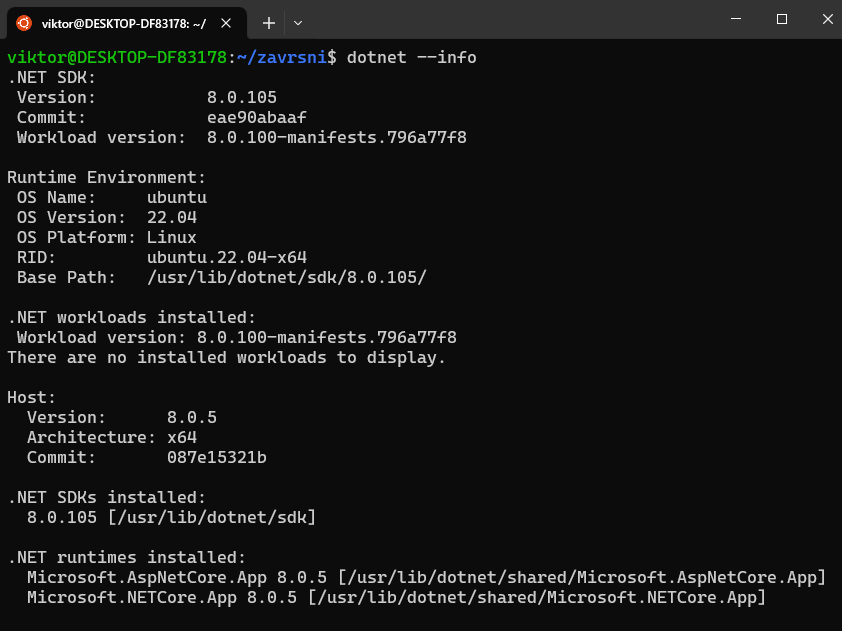
\includegraphics[width=0.9\textwidth]{slike/info.png}
    \caption{.NET informacije (Izvor: autor)}
    \label{fig:info}
\end{figure}
\vspace{12pt}
Za dodatnu provjeru možemo pokrenuti osnovni program koji će ispisati "Hello World" na ekran sa naredbama\cite{nettest}:

\begin{lstlisting}[language=bash]
dotnet new console -o aplikacija
cd aplikacija
dotnet run
\end{lstlisting}

\section{Primjer}
Slična domena problema kao i kod primjera Bash skripte, za primjer .NET skripte sam odlučio napraviti nadzor za status stranica tako što sam napravio prvu skriptu koja služi kao poslužitelj, a druga skripta provjerava stanje tog poslužitelja. U prvoj se skripti na liniji \textbf{1} specificira korištenje \textit{Net} biblioteke iz korijenske biblioteke \textit{System}. Linija \textbf{3} definira klasu Emulator, a linija \textbf{5} definira glavnu funkciju koja je asinkrona. Na liniji \textbf{7} se definira port na kojemu želimo posluživati, linija \textbf{9} stvara novi objekt klase \verb|HttpListener| kojemu se u liniji \textbf{11} u polje dodaje URL do servisa i na liniji \textbf{12} pokreće slušanje za zahtjeve na tom URL-u. U beskonačnoj petlji na liniji \textbf{16} se na liniji \textbf{18} u objekt klase \verb|HttpListenerContext| sprema zahtjev koji dođe na poslužitelj te se kroz linije \textbf{20}, \textbf{21} i \textbf{22} odgovara na zahtjev sa kodom 200. Na linijama \textbf{24} i \textbf{25} skripta zatim ispisuje da je primila zahtjev i trenutno vrijeme. Važno je napomenuti da zbog asinkronog izvođenja slušanja na zahtjeve će se kod u beskonačnoj petlji odviti tek kada dođe neki zahtjev.

\begin{lstlisting}[language=C++]
1  using System.Net;
2
3  class Emulator
4  {
5      static async Task Main(string[] args)
6      {
7          int port = 8080;
8
9          using (HttpListener slusac = new HttpListener())
10         {
11             slusac.Prefixes.Add($"http://localhost:{port}/");
12             slusac.Start();
13
14             Console.WriteLine($"Slusam port:{port}...");
15
16             while (true)
17             {
18                 HttpListenerContext kontekst = await slusac.GetContextAsync();
19
20                 kontekst.Response.StatusCode = 200;
21                 kontekst.Response.StatusDescription = "OK";
22                 kontekst.Response.Close();
23
24                 string vrijeme = DateTime.Now.ToString("yyyy-MM-dd HH:mm:ss");
25                 Console.WriteLine($"{vrijeme} Primio zahtjev, odgovorio");
26             }
27         }
28     }
29 }
\end{lstlisting}

Druga skripta je zapravo glavna skripta koja provjerava jesu li neke stranice dostupne ili ne, tj. služi za nadzor u slučaju da stranica postane nedostupna ili se vrati kao dostupna. Glavna klasa se zove \verb|StatusMonitor|, na liniji \textbf{3} se definira objekt tipa riječnik što je struktura podataka koja u ovom slučaju prima jedan znakovni niz i jednu boolean vrijednost gdje boolean vrijednost služi za postavljanje inicijalnog stanja stranice. Na liniji \textbf{4} se definira interval što je objekt tipa klase \verb|TimeSpan|. Na linijama \textbf{8} i \textbf{9} se u spomenuti riječnik stavljaju stranice nad kojima se vrši nadzor, što su u ovom slučaju "stranica" koju prva skripta poslužuje i \textit{www.google.com}. U beskonačnoj petlji se za svaku promatranu stranicu na liniji \textbf{17} poziva asinkrona funkcija \verb|ProvjeriAsync| koja se nalazi na liniji \textbf{33}. Ova funkcija šalje zahtjev poslužitelju i ako dobije odgovor 200 na liniji \textbf{42} vraća istinitu vrijednost, a u suprotnom vraća lažnu vrijednost. Na liniji \textbf{20} se prethodni status stranice uspoređuje sa novodobivenim te ako nisu isti onda se pokazuje novi status stranice time što se na liniji \textbf{25} poziva funkcija \verb|Obavijesti| koja na terminal ispisuje trenutno vrijeme, stranicu i njen novi status tj. radi li ili ne. Na liniji \textbf{29} se postavlja "spavanje" dretve na 5 sekundi prije nego opet ponovi korake beskonačne petlje.

\begin{lstlisting}[language=C++]
1  class StatusMonitor
2  {
3      private static Dictionary<string, bool> statusStranice = new Dictionary<string, bool>();
4      private static TimeSpan interval = TimeSpan.FromSeconds(5);
5
6      static async Task Main(string[] args)
7      {
8          statusStranice.Add("http://localhost:8080", true);
9          statusStranice.Add("www.google.com", true);
10
11         Console.WriteLine("Promatram:");
12
13         while (true)
14         {
15             foreach (var stranica in statusStranice.Keys)
16             {
17                 bool status = await ProvjeriAsync(stranica);
18                 bool prethodniStatus = statusStranice[stranica];
19
20                 if (status != prethodniStatus)
21                 {
22                     statusStranice[stranica] = status;
23                     string statusPoruka = status ? "radi" : "ne radi";
24
25                     Obavijesti(stranica, statusPoruka);
26                 }
27             }
28
29             Thread.Sleep(interval);
30         }
31     }
32
33     static async Task<bool> ProvjeriAsync(string url)
34     {
35         try
36         {
37             using (HttpClient client = new HttpClient())
38             {
39                 client.Timeout = TimeSpan.FromSeconds(5);
40
41                 HttpResponseMessage response = await client.GetAsync(url);
42                 return response.IsSuccessStatusCode;
43             }
44         }
45         catch
46         {
47             return false;
48         }
49     }
50
51     static void Obavijesti(string website, string status)
52     {
53         string currentTime = DateTime.Now.ToString("yyyy-MM-dd HH:mm:ss");
54         Console.WriteLine($"{currentTime} {website} {status}");
55     }
56 }
\end{lstlisting}
Na slici \ref{fig:netprimjer} se vidi rad obje skripte. Nakon pokretanja obje skripte, skripta StatusMonitor šalje zahtjeve u 12:07:25 12:07:31 i 12:07:36 na koje skripta Emulator odgovora. Nakon gašenja skripte Emulator i time gašenja poslužitelja, u 12:07:42 skripta StatusMonitor obaviještava o nedostupnosti poslužitelja, te ponovnim paljenjem skripte Emulator skripta StatusMonitor u 12:07:47 obaviještava da je poslužitelj postao dostupan.
\begin{figure}[H]
    \centering
    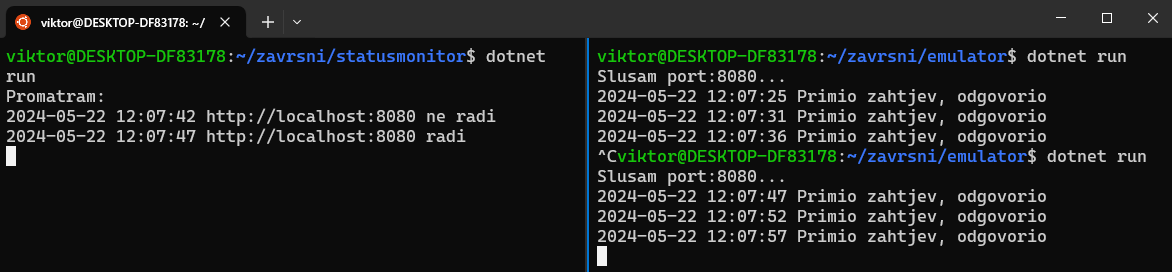
\includegraphics[width=1.1\textwidth]{slike/netprimjer.png}
    \caption{Rad obje .NET skripte (Izvor: autor)}
    \label{fig:netprimjer}
\end{figure}

\chapter{dotnet-script i dotnet-shell}
\textbf{dotnet-script} je .NET alat koji omogućava vrlo jednostavno korištenje .NET skripti, tj. eliminira potrebnu za stvaranjem cijelog projekta kao što se to radilo na prethodnom primjeru gdje se skripta morala pokrenuti sa \verb|dotnet run| (Slika \ref{fig:netprimjer}). Također podržava i "interaktivni" način rada gdje se C\# kod može izvršavati direktno u terminalu i mogu se koristiti NuGet paketi koji se vežu za sesiju, tj. nisu trajno preuzeti. Ako je instalirana .NET SDK verzija 6,7 ili 8 tada se dotnet-script može instalirati naredbom\cite{gitscript}:
\begin{lstlisting}[language=C++]
dotnet tool install -g dotnet-script
\end{lstlisting}
C\# skripte završavaju sa .csx nastavkom i pokreću se naredbom \verb|dotnet-script|. Ako imamo skriptu zvanu "skripta.csx" tada ju pokrećemo naredbom \verb|dotnet-script skripta.csx|. Kako bi se olakšalo pokretanje skripte, u skriptu se može dodati shebang linija \texttt{\#!/usr/bin/env dotnet-script} te nakon mijenjanja prava skripte sa \verb|chmod u+x skripta.csx| skripta se može pokrenuti sa jednostavnim \verb|./skripta.csx| kao i obične Bash skripte. Skripti se također standardno prenose argumenti tako što ih navedemo u istoj liniji u kojoj pozivamo skriptu. Kao što je spomenuto, u skriptama se mogu koristiti u NuGet paketi sa sintaksom \verb|#r "nuget: ime, verzija"|. Skripte se mogu i učitati u druge skripte sa \verb|#load| direktivom što omogućuje bolju organizaciju i modularnost skripti\cite{gitscript}.
dotnet-script također sadrži interaktivni tj. REPL (engl. \textit{Read-Evaluate-Print-Loop}) način rada. Ovaj način rada se pokreće naredbom \verb|dotnet-script| nakon čega mogu upisivati linije C\# koda koje se odmah izvršavaju\cite{gitscript}. 
\begin{figure}[H]
    \centering
    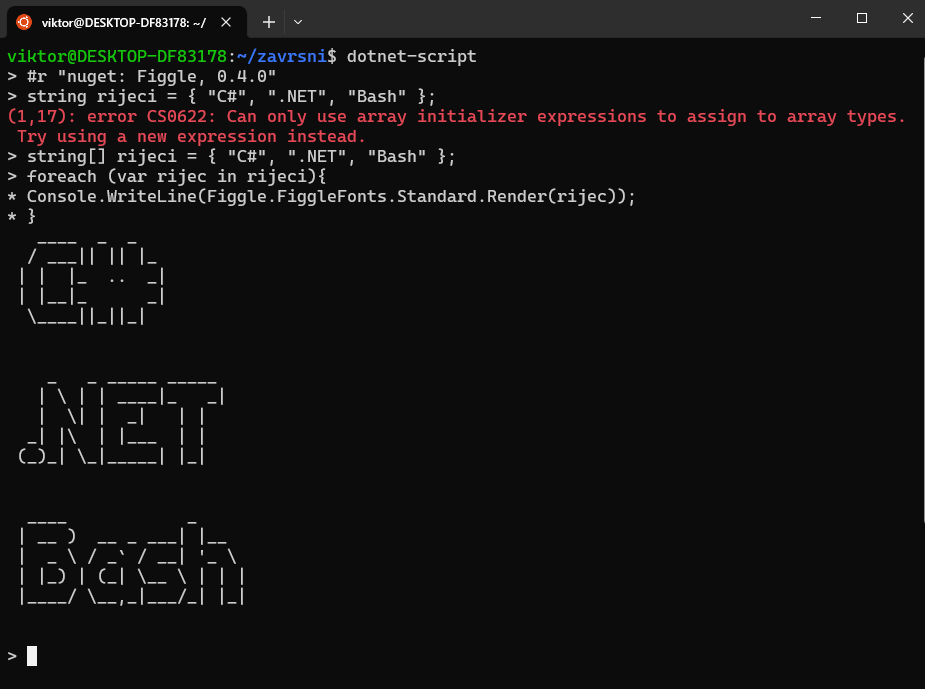
\includegraphics[width=0.9\textwidth]{slike/script-repl.png}
    \caption{Demonstracija interaktivnog načina rada dotnet-script (Izvor: autor)}
    \label{fig:script-repl}
\end{figure}
Na slici \ref{fig:script-repl} je demonstrirano korištenje interaktivnog načina gdje se referencira NuGet paket "Figgle", stvara polje riječi i ispisuje ukrašeni prikaz tih riječi korištenjem biblioteke. Također je pokazan i prikaz poruka pogreške. Važno je ponovno napomenuti kako su referencirani NuGet paketi vezani samo uz trenutnu sesiju, što znači da kada se izađe sa \verb|#exit| ili CTRL+C i ponovno stvori sesija sa \verb|dotnet-shell| paket više neće biti dostupan.
Da zaključim, dotnet-script je odličan alat za jednostavno izvršavanje napisanih C\# skripti i isprobavanje koda u interaktivnom načinu rada jer podržava višelinijsko pisanje koda direktno u terminalu.

\textbf{dotnet-shell} je meta ljuska koja se izvršava na postojećoj ljuski, bilo to Bash/PowerShell ili neka druga. dotnet-shell je nastao nakon dotnet-scripta pa nadograđuje na brojne njene koncepte i mogućnosti, ali i dijeli puno njih. Poput dotnet-script, dotnet-shell može jednostavno izvršavati C\# skripte, no sada su sa ekstenzijom .nsh, može koristiti NuGet pakete i učitavati skripte sa \verb|#load|. Najveća razlika je što je dotnet-shell, kao što i ime upućuje, sličnije ljusci nego nego samo alatu za pisanje skripti. To je iz razloga što se na njegovom naredbenom retku mogu izvršavati i Bash i C\# linije te kombinirati sa tehnikom "hvatanja" izlaza Bash naredbe koristeći `` simbole. Bash skripte se također mogu pokretati unutar .nsh skripti koristeći \verb|Process| objekt, no to utječe na interoperabilnost skripti. Ako imamo instaliranu .NET verziju 6,7 ili 8 tada se dotnet-shell može instalirati sa naredbom\cite{gitshell}:
\begin{lstlisting}[language=C++]
dotnet tool install -g dotnet-shell
\end{lstlisting}
S obzirom da dotnet-shell dijeli elemente dotnet-scripta, neću ih ponovno spominjati. Najveća razlika u korištenju dotnet-shella je što .nsh skripte mogu sadržavati i C\# kod i Bash naredbe koje se izvršavaju bez problema. Također, u interaktivnom načinu rada u koji se ulazi sa naredbom \verb|dotnet-shell| se ne može pisati višelinijski kod poput petlji kao što se to može u dotnet-scrip alatu. Zbog kombiniranja Bash naredbi i C\# sintakse u skriptama je dotnet-shell vrlo moćan alat za jednostavno korištenje vrlo kompleksnih skripti.

Za primjer .nsh skripte sam napravio skriptu koja spaja više PDF datoteka u jednu PDF datoteku. Linija \textbf{1} je referenciranje NuGet paketa koji je potreban za operacije. Linije \textbf{3} do \textbf{7} uključuju potrebne biblioteke, od kojih su i referencirane NuGet paket biblioteke. Na liniji \textbf{9} se stvara instanca klase "Encoding" koristeći \verb|CodePagesEncodingProvider| i sa metodom \verb|GetEncoding(1252)| se vraća objekt za format kodiranja koristeći Windows-1252 kodiranje znakova. U liniji \textbf{10} se instanca \verb|CodePagesEncodingProvider| registrira sa \verb|Encoding| klasom čime skripta dobiva pristup kodiranju i dekodiraju teksta koristeći Windows-1252 kodiranje znakova. Na liniji \textbf{30} se određuje putanja do direktorija gdje se nalaze PDF datoteke, ovdje je postavljeno da je to isti direktorij gdje se nalazi i skripta. Na liniji \textbf{31} se postavlja ime datoteke koja će sadržavati sve spojene PDF datoteke. Linija \textbf{32} koristi \verb|Directory| statičnu klasu iz \verb|System.IO| .NET biblioteke i \verb|GetFiles| metodu koja vraća putanje datoteka koje odgovaraju nekom danom uzorku, u ovom slučaju sve datoteke koje završavaju sa ".pdf". Na liniji \textbf{34} se provjerava postoji li ijedna PDF datoteka, ako ne postoji ispisuje se poruka. Na liniji \textbf{40} se prolazi kroz svaki zapis u polju svih datoteka i ispisuju se putanje svih nađenih PDF datoteka. Na liniji \textbf{44} se poziva funkcija \verb|SpojiPDFove| kojoj se prenosi polje datoteka, tj. putanja, i putanja izlazne datoteke. Na liniji \textbf{14} se stvara novi objekt klase \verb|PdfDocument| zvan "spojeniDokument". Zatim se prolazi kroz svaku nađenu PDF datoteku i koristeći \verb|Open| metodu klase \verb|PdfReader| se PDF datoteka učitava u varijablu \verb|ulazniPDF| nakon čega se svaka stranica tog PDF-a dodaje objektu \verb|spojeniDokument|, tj. PDF datoteci koja će sadržavati sve stranice svih PDF datoteka. Na kraju dodavanja svih stranica novom dokumentu se na liniji \textbf{26} sprema PDF koji sadrži sve PDF-ove spojene u sebe.

\begin{lstlisting}[language=C++]
1: #r "nuget: PdfSharp, 1.50.5147"
2:
3: using System;
4: using System.IO;
5: using PdfSharp.Pdf;
6: using PdfSharp.Pdf.IO;
7: using System.Text;
8:
9: var enc = CodePagesEncodingProvider.Instance.GetEncoding(1252);
10: Encoding.RegisterProvider(CodePagesEncodingProvider.Instance);
11:
12: void SpojiPDFove(string[] pdfDatoteke, string putanjaIspis)
13: {
14:     using (var spojeniDokument = new PdfDocument())
15:     {
16:         foreach(var datoteka in pdfDatoteke)
17:         {
18:             using (var ulazniPdf = PdfReader.Open(datoteka, PdfDocumentOpenMode.Import))
19:             {
20:                 foreach (var stranica in ulazniPdf.Pages)
21:                 {
22:                     spojeniDokument.AddPage(stranica);
23:                 }
24:             }
25:         }
26:         spojeniDokument.Save(putanjaIspis);
27:     }
28: }
29:
30: string pdfDirektorij = ".";
31: string spojeniPdf = "MergedOutput.pdf";
32: string[] pdfDatoteke = Directory.GetFiles(pdfDirektorij, "*.pdf");
33:
34: if (pdfDatoteke.Length == 0)
35: {
36:     Console.WriteLine("Nema PDF datoteka u trenutnom direktoriju.");
37: }
38: else
39: {
40:     foreach (var datoteka in pdfDatoteke)
41:     {
42:         Console.WriteLine(datoteka);
43:     }
44:     SpojiPDFove(pdfDatoteke, spojeniPdf);
45:     Console.WriteLine($"PDF-ovi spojeni u {spojeniPdf}");
46: }
\end{lstlisting}

\begin{figure}[H]
    \centering
    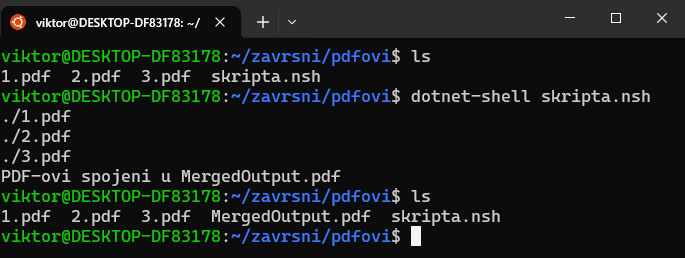
\includegraphics[width=0.9\textwidth]{slike/pdflinux.png}
    \caption{Ispis skripte za spajanje PDF datoteka (Izvor: autor)}
    \label{fig:pdflinux}
\end{figure}

\chapter{Interoperabilnost}
Kao što je to prijašnje obrađeno u radu, najveća prednost korištenja .NET tehnologije za pisanje skripti je interoperabilnost između operacijskih sustava. Demonstrirati ću interoperabilnost na primjeru prethodno pokazane skripte za spajanje PDF datoteka. Na Windows operacijskom sustavu se .NET može instalirati korištenjem PowerShell ljuske sa naredbom\cite{windowsdotnet}:
\begin{lstlisting}[language=C++]
winget install Microsoft.DotNet.SDK.8
\end{lstlisting}
Nakon toga se dotnet-shell može instalirati istom naredbom kao i prethodno jer se koristi dotnet CLI.
Nakon što PDF datoteke stavimo u isti direktorij kao i skriptu, skripta se standardno pokreće sa \verb|dotnet-shell .\skripta.nsh| nakon čega se PDF datoteke ispravno spajaju u jednu datoteku (Slika \ref{fig:pdfws}).

\begin{figure}[H]
    \centering
    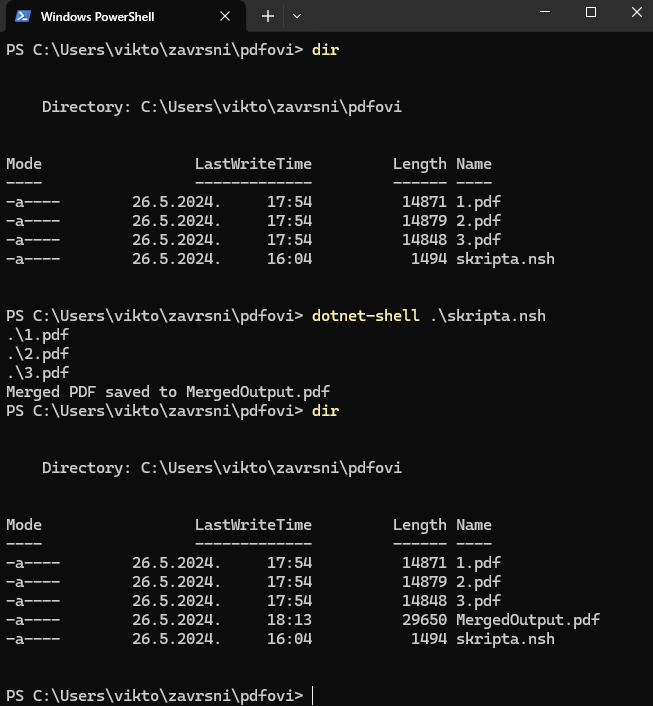
\includegraphics[width=0.9\textwidth]{slike/pdfwindows.png}
    \caption{Ista skripta na Windows OS-u (Izvor: autor)}
    \label{fig:pdfws}
\end{figure}

\chapter{Usporedba prednosti i nedostataka .NET skripti i klasičnih shell skripti}
Kako bih direktno usporedio pisanje .NET skripti i Bash skripti, primjer Bash skripte iz poglavlja \textbf{5.6} (Slika \ref{fig:primjerbash}) ću napisati u .NET-u koristeći C\#, a primjer .NET skripte iz poglavlja \textbf{6.2} (Slika \ref{fig:netprimjer}) u Bash skriptnom jeziku i usporediti ih.
\section{Bash skripta kao .NET skripta}
Prva skripta iz primjera Bash skripti u poglavlju \textbf{5.6} je u .NET-u sljedeća:
\begin{lstlisting}[language=C++]
1   using System;
2   using System.IO;
3   using System.Threading;
4   
5   var log = "server.log";
6   
7   void Generiraj()
8   {
9       var vrste = new string[] { "INFO", "WARN", "ERROR" };
10      var vrsta = vrste[new Random().Next(0, vrste.Length)];
11      var poruka = $"Poruka tipa: {vrsta}";
12      File.AppendAllText(log, $"{DateTime.Now:yyyy-MM-dd HH:mm:ss} {vrsta}: {poruka}\n");
13  }
14  
15  while (true)
16  {
17      Generiraj();
18      Thread.Sleep(new Random().Next(1000, 5000));
19  }
\end{lstlisting}
Zbog jednostavnosti skripte nema velikih razlika između skripti, gotovo su identične od linije do linije i obje skripte su jednostavne za razumjeti i čitljive. Druga skripta iz primjera Bash skripti je u .NET-u sljedeća:
\begin{lstlisting}[language=C++]
 1   #r "nuget: Colorful.Console, 1.2.8"
 2   
 3   using System;
 4   using System.IO;
 5   using System.Threading;
 6   using System.Linq;
 7   using Colorful;
 8   using System.Drawing;
 9   
10   var log = "server.log";
11   var temp = ".temp_datoteka";
12   
13   void Analiziraj()
14   {
15       int zadnjaPozicija = 0;
16       if (File.Exists(temp))
17       {
18           zadnjaPozicija = int.Parse(File.ReadAllText(temp));
19       }
20   
21       int brojLinijaLog = 0;
22       if (File.Exists(log))
23       {
24           brojLinijaLog = File.ReadAllLines(log).Length;
25       }
26   
27       if (brojLinijaLog < zadnjaPozicija)
28       {
29           zadnjaPozicija = 0;
30       }
31   
32       var novo = string.Join("\n", File.ReadAllLines(log).Skip(zadnjaPozicija));
33   
34       if (!string.IsNullOrEmpty(novo))
35       {
36           foreach (var linija in novo.Split('\n'))
37           {
38               if (linija.Contains("WARN") || linija.Contains("ERROR"))
39               {
40                   var styleSheet = new StyleSheet(Color.White);
41                   if (linija.Contains("WARN"))
42                   {
43                       styleSheet.AddStyle("WARN", Color.Yellow);
44                   }
45                   else if (linija.Contains("ERROR"))
46                   {
47                       styleSheet.AddStyle("ERROR", Color.Red);
48                   }
49                   Colorful.Console.WriteLineStyled(linija, styleSheet);
50               }
51           }
52       }
53   
54       File.WriteAllText(temp, brojLinijaLog.ToString());
55   }
56   
57   while (true)
58   {
59       Analiziraj();
60       Thread.Sleep(1000);
61   }
\end{lstlisting}
Od linije \textbf{10} do linije \textbf{32} je skripta otprilike identična Bash skripti, s jedinom iznimkom što je primjerice iz \verb|int.Parse| vidljivije da se očekuje broj u \verb|temp| datoteci, dok u Bash verziji sa samo \verb|cat $temp| to nije vidljivo. Prva najveća razlika se vidi u liniji \textbf{32} naspram Bash linije \textbf{25} u tome što je C\# linija puno čitljivija i prati način cjevovoda kojeg koriste većina programskih jezika. Bash linija koda koristi substituciju naredbi \verb|$((zadnja_pozicija + 1))| što je aritmetička operacija koju zatim dodjeljuje naredbi \verb|tail| koja se primjenjuje na datoteku u varijabli \verb|log| kako bi isčitala sve linije od dane pozicije, a sve to se nalazi u substituciji naredbe koja svoj izlaz sprema u varijablu \verb|novo|. Slično tome, na duži no čitljiviji način C\# linija koristi \verb|File.ReadAllLines| kako bi pročitala linije \verb|log| datoteke, koristi metodu \verb|Skip| kako bi se pozicionirala na željenu liniju i to se sve daje kao argument metodi \verb|Join| koja parsira linije koristeći \verb|\n| kao simbol za novi red. Iako je Bash linija kraća, na prvi pogled je C\# linija puno lakša za shvatiti slijed cjevovoda. Linije \textbf{36} do \textbf{54} obavljaju istu funkciju kao linije \textbf{27} do \textbf{37} Bash skripte, no sa malom izmjenom. Koristi se NuGet paket "Colorful.Console" uz pomoć kojega se puno lakše ispisuju boje na terminal jer nije potrebno raditi sa ANSI \textit{escape code}-om nego je dovoljno samo napisati ime boje. Također, iako nije tako implementirano u Bash skripti, u C\# skripti se boje primjenjuju samo na riječi "WARN" I "ERROR" jednostavnom metodom \verb|AddStyle| koja na dani uzorak primjenjuje boju, dok bi se u Bash skripti za tu funkcionalnost morao pisati regularni izraz poput \verb+s/WARN/${ZUTA}WARN${BIJELA}/g+ koji je manje čitljiv. Zadnja veća razlika skripti je linija \textbf{54} u kojoj je lako čitljivo da se koristeći metodu \verb|WriteAllText| u datoteku spremljenu u varijabli \verb|temp| sprema broj linija, dok je u Bash skripti ta linija sljedeća: \texttt{wc -l < \$log > \$temp} i osobi koja nije iskusna sa preusmjeravanjem standardnog izlaza može biti zbunjujući poredak ulaza i izlaza, tj. cjevovoda. Da zaključim, u primjeru ove dvije skripte nema velikih razlika između Bash i .NET C\# skripti, no C\# skripte su čitljivije i pružaju veću razinu apstrakcije koristeći metode iz biblioteka ili referenciranih NuGet paketa.

\begin{figure}[H]
    \centering
    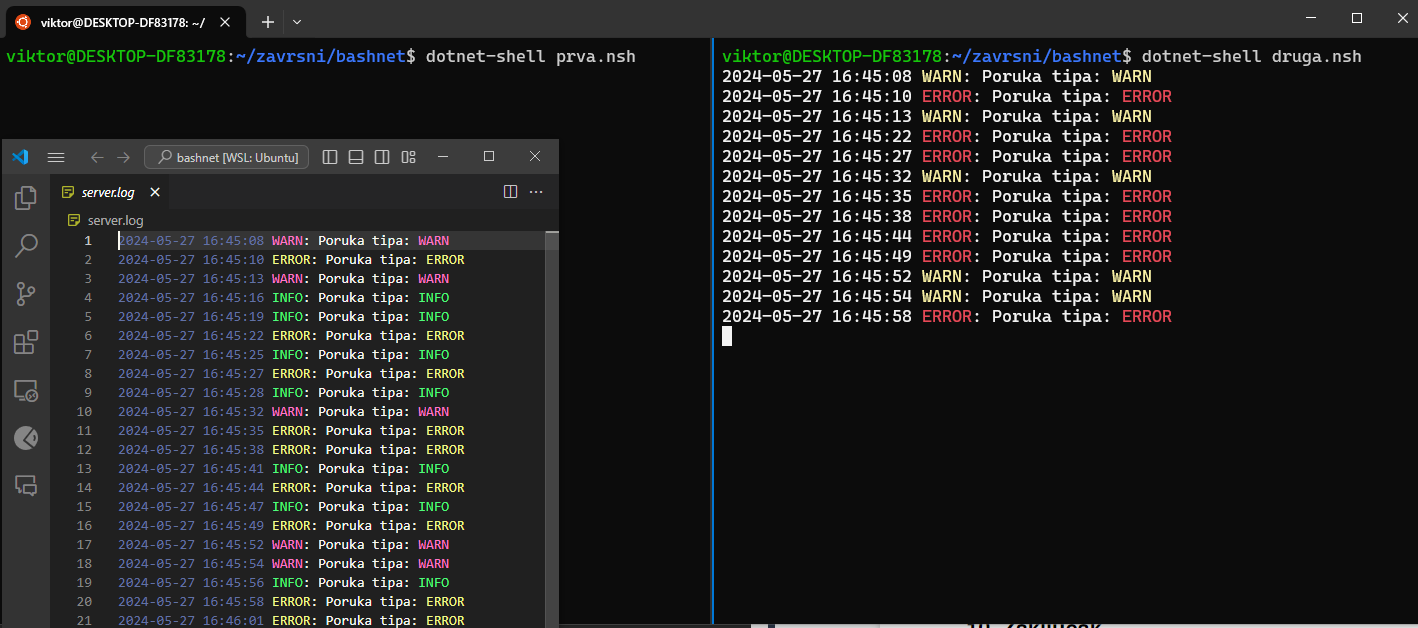
\includegraphics[width=1\textwidth]{slike/bashunet.png}
    \caption{Rad konvertirane .NET skripte (Izvor: autor)}
    \label{fig:bashunet}
\end{figure}
\section{.NET skripta kao Bash skripta}
Prva skripta iz .NET primjera skripti je služila za podizanje poslužitelja i jednostavno odgovaranje na zahtjeve. Ta je skripta u Bash jeziku sljedeća:
\begin{lstlisting}[language=bash]
1   #!/bin/bash
2
3   PORT=8080
4   echo "Slusam port: $PORT..."
5   HTTP_ODGOVOR="HTTP/1.1 200 OK\r\nContent-Length: 0\r\n\r\n"
6
7   while true; do
8       {
9           echo -ne "$HTTP_ODGOVOR"
10       } | nc -l -s 127.0.0.1 -p "$PORT" > /dev/null 2>&1
11
12      VRIJEME=$(date +"%Y-%m-%d %H:%M:%S")
13      echo "$VRIJEME Primio zahtjev, odgovorio"
14  done

\end{lstlisting}
Ova je skripta na prvi pogled dva puta kraća od .NET varijante, no cijena toga je čitljivost. Na liniji \textbf{5} se definira HTTP odgovor koji će se vratiti zahtjevu, a to je 200 OK. Koristeći znak za novu liniju \verb|\n| i znak \verb|\r| se pridržava standardu HTTP/1.1. standarda. U beskonačnoj petlji naredba \verb|echo -ne "$HTTP_ODGOVOR"| šalje HTTP odgovor cjevovodom u netcat naredbu. Koriste se argumenti \verb|n| kako echo ne bi dodao novu liniju i \verb|e| kako bi se znakovi \verb|\n| i \verb|\r| tretirali kao specijalni znakovi, a ne tekst. HTTP odgovor se mogao direktno dati naredbi \verb|echo| no radi preglednosti sam ga spremio u varijablu. Alat netcat se poziva naredbom \verb|nc|, a daje mu se argument \verb|-l| kako bi bio u načinu rada za slušanje i argument \verb|-s| s kojim se specificira izvor, tj. localhost u ovom slučaju. Argument \verb|-p| specificira port iz varijable \verb|$PORT|, a argument \verb|-q 1| se koristi kako netcat ne bi ispisivao svoje poruke na standardni izlaz što bi ga popunilo. Standardni izlaz se preusmjerava u \verb|/dev/null| čime se zapravo briše, a \verb|2>&1| preusmjerava poruke pogreške na isto mjesto. Ostatak koda je gotovo identičan .NET verziji.

Druga skripta je služila za slanje zahtjeva i provjeravanje je li se status stranice promijenio.
\begin{lstlisting}[language=bash]
1   #!/bin/bash
2   
3   declare -A statusStranice
4   statusStranice["http://localhost:8080"]=1
5   statusStranice["https://www.google.com"]=1
6   
7   interval=5
8   
9   echo "Promatram:"
10  
11  while true; do
12      for stranica in "${!statusStranice[@]}"; do
13          status=$(curl -s -o /dev/null -w "%{http_code}" "$stranica")
14          prethodniStatus=${statusStranice[$stranica]}
15          
16          if [ "$status" -eq 200 ]; then
17              noviStatus=1
18          else
19              noviStatus=0
20          fi
21  
22          if [ "$noviStatus" -ne "$prethodniStatus" ]; then
23              statusStranice[$stranica]=$noviStatus
24              if [ "$noviStatus" -eq 1 ]; then
25                  statusPoruka="radi"
26              else
27                  statusPoruka="ne radi"
28              fi
29              currentTime=$(date +"%Y-%m-%d %H:%M:%S")
30              echo "$currentTime $stranica $statusPoruka"
31          fi
32      done
33      sleep $interval
34  done
\end{lstlisting}
Ova skripta je gotovo identična .NET skripti, no najveća razlika je u liniji \textbf{13} u kojoj se koristeći \verb|curl| alat sa argumentom \verb|-s| kojim se označava da curl ne ispisuje svoje interne poruke, argumentom \verb|-o| koji šalje tijelo odgovora u \verb|/dev/null| čime se on efektivno briše i argumentom \verb|-w "%{http_code}"| kojim se curl naredbi daje format da ispisuje samo kod odgovora i konačno se kroz varijablu \verb|stranica| curl naredbi daje adresa poslužitelja, tj. stranice. Ostatak skripte je prilično slična .NET skripti jer se provjerava status i je li drugačiji od prošlog statusa.
\begin{figure}[H]
    \centering
    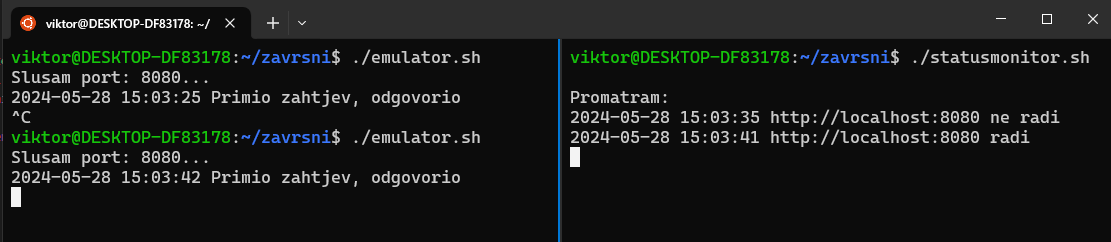
\includegraphics[width=1\textwidth]{slike/netubash.png}
    \caption{Rad konvertirane Bash skripte (Izvor: autor)}
    \label{fig:netubash}
\end{figure}
Za razliku od prvog primjera konvertiranja Bash skripte u .NET skriptu, ovo konvertiranje predstavlja neke sigurnosne probleme. Bash verzija skripte koristi netcat alat koji je nisko razinski alat naspram .NET HttpListener klase koja implementira razne sigurnosne funkcionalnosti. Također, velika razlika je upravljanje pogreškama jer HttpListener ima puno ekstenzivnije upravljanje pogreškama nego netcat alat.

Da sumiram, Bash skripte su nešto kraće i koriste alate koji su dostupni u gotovo svim GNU/Linux distribucijama bez potrebe za dodatnim instaliranjem ikakvih alata ili tehnologija poput .NET-a što im daje veliku portabilnost, no nasuprot tome .NET skripte omogućavaju korištenje ogromnog broja NuGet biblioteka i standardnih .NET biblioteka koje imaju unaprijed razrađene funkcionalnosti i sigurnosne mjere te ih osoba koja piše skriptu ne mora razvijati od početka. Osim toga, skripte su interoperabilne na svim operacijskim sustavima koji imaju .NET instaliran što im daje veliku prednost. Još jedna prednost .NET skripti su čitljivost zbog standardnijeg C\# koda koji prati vrlo poznatu sintaksu Java jezika i donekle C/C++ jezika.
\chapter{Zaključak}
.NET okruženje za skriptiranje u GNU/Linux naredbenom retku pruža nove mogućnosti za razvoj i automatizaciju. Kroz rad je demonstriran veći broj Bash i .NET skripti i demonstrirana je integracija .NET alata i Bash ljuske koristeći .NET alat dotnet-shell. Kroz primjere su prikazane prednosti i nedostatci oba sustava. .NET poboljšava interoperabilnost time što se skripte mogu direktno koristiti na svim operacijskim sustavima koji imaju instalirano .NET okruženje. Također, .NET pruža dodatne funkcionalnosti preko svojih biblioteka i NuGet paketa što omogućuje jednostavno razvijanje kompleksnijih skripti čime se još više mogu poboljšati radni procesi. Prednost Bash skripti je što rade na svim GNU/Linux distribucijama koje koriste Bash ljusku bez potrebe za dodatnim instalacijama i zahtjevaju manje resursa od .NET skripti čime su lakše za sustave. Da zaključim, sinergija .NET okruženja i Bash skriptnog jezika u GNU/Linux operacijskom sustavu omogućuje moćno okruženje za projekte automatizacije iz razloga što se može koristiti najbolje od oba jezika pri pisanju skripti, .NET elementi za kompleksne unaprijed pripremljene funkcionalnosti, a Bash za GNU/Linux specifične radnje ukoliko ima potrebe za njima. 


\printbibliography[title=Popis literature]
\addcontentsline{toc}{chapter}{Popis literature}

\listoffigures
\addcontentsline{toc}{chapter}{Popis slika}

\listoftables
\addcontentsline{toc}{chapter}{Popis tablica}

\end{document}
